\documentclass[]{article}
\usepackage{lmodern}
\usepackage{amssymb,amsmath}
\usepackage{ifxetex,ifluatex}
\usepackage{fixltx2e} % provides \textsubscript
\ifnum 0\ifxetex 1\fi\ifluatex 1\fi=0 % if pdftex
  \usepackage[T1]{fontenc}
  \usepackage[utf8]{inputenc}
\else % if luatex or xelatex
  \ifxetex
    \usepackage{mathspec}
  \else
    \usepackage{fontspec}
  \fi
  \defaultfontfeatures{Ligatures=TeX,Scale=MatchLowercase}
\fi
% use upquote if available, for straight quotes in verbatim environments
\IfFileExists{upquote.sty}{\usepackage{upquote}}{}
% use microtype if available
\IfFileExists{microtype.sty}{%
\usepackage{microtype}
\UseMicrotypeSet[protrusion]{basicmath} % disable protrusion for tt fonts
}{}
\usepackage[margin=1in]{geometry}
\usepackage{hyperref}
\hypersetup{unicode=true,
            pdftitle={Standardization \& Balancing Overall Workflow of the new methodology},
            pdfauthor={Cristina Muschitiello Food and Agriculture Organization of the United Nations},
            pdfborder={0 0 0},
            breaklinks=true}
\urlstyle{same}  % don't use monospace font for urls
\usepackage{longtable,booktabs}
\usepackage{graphicx,grffile}
\makeatletter
\def\maxwidth{\ifdim\Gin@nat@width>\linewidth\linewidth\else\Gin@nat@width\fi}
\def\maxheight{\ifdim\Gin@nat@height>\textheight\textheight\else\Gin@nat@height\fi}
\makeatother
% Scale images if necessary, so that they will not overflow the page
% margins by default, and it is still possible to overwrite the defaults
% using explicit options in \includegraphics[width, height, ...]{}
\setkeys{Gin}{width=\maxwidth,height=\maxheight,keepaspectratio}
\IfFileExists{parskip.sty}{%
\usepackage{parskip}
}{% else
\setlength{\parindent}{0pt}
\setlength{\parskip}{6pt plus 2pt minus 1pt}
}
\setlength{\emergencystretch}{3em}  % prevent overfull lines
\providecommand{\tightlist}{%
  \setlength{\itemsep}{0pt}\setlength{\parskip}{0pt}}
\setcounter{secnumdepth}{5}
% Redefines (sub)paragraphs to behave more like sections
\ifx\paragraph\undefined\else
\let\oldparagraph\paragraph
\renewcommand{\paragraph}[1]{\oldparagraph{#1}\mbox{}}
\fi
\ifx\subparagraph\undefined\else
\let\oldsubparagraph\subparagraph
\renewcommand{\subparagraph}[1]{\oldsubparagraph{#1}\mbox{}}
\fi

%%% Use protect on footnotes to avoid problems with footnotes in titles
\let\rmarkdownfootnote\footnote%
\def\footnote{\protect\rmarkdownfootnote}

%%% Change title format to be more compact
\usepackage{titling}

% Create subtitle command for use in maketitle
\newcommand{\subtitle}[1]{
  \posttitle{
    \begin{center}\large#1\end{center}
    }
}

\setlength{\droptitle}{-2em}
  \title{Standardization \& Balancing\\
Overall Workflow of the new methodology}
  \pretitle{\vspace{\droptitle}\centering\huge}
  \posttitle{\par}
  \author{Cristina Muschitiello\\
Food and Agriculture Organization of the United Nations}
  \preauthor{\centering\large\emph}
  \postauthor{\par}
  \predate{\centering\large\emph}
  \postdate{\par}
  \date{17 May 2018}

\usepackage{lscape}
\usepackage{booktabs}
\usepackage{longtable}
\usepackage{array}
\usepackage{multirow}
\usepackage[table]{xcolor}
\usepackage{wrapfig}
\usepackage{float}
\usepackage{colortbl}
\usepackage{pdflscape}
\usepackage{tabu}
\usepackage{threeparttable}
\usepackage{threeparttablex}
\usepackage[normalem]{ulem}
\usepackage{makecell}

\usepackage{draftwatermark}
\usepackage{makeidx}
\makeindex
\usepackage{float}
\floatplacement{figure}{H}
\usepackage{amsmath}
\usepackage{amssymb}
\usepackage{amsthm}
\usepackage{mathtools}

\begin{document}
\maketitle
\begin{abstract}
This vignette provides a description of the Workflow of the
Standardization and Balancing Procedure: This represents the process of
aggregating and balancing all the accounts of individual products to
their primary equivalents. Other documents will provide details of each
step of the overall procedure.
\end{abstract}

{
\setcounter{tocdepth}{4}
\tableofcontents
}
\subsection*{Disclaimer}\label{disclaimer}
\addcontentsline{toc}{subsection}{Disclaimer}

This Working Paper should not be reported as representing the official
view of the FAO. The views expressed in this Working Paper are those of
the author and do not necessarily represent those of the FAO or FAO
policy. Working Papers describe research in progress by the authors and
are published to elicit comments and to further discussion.

This paper is dynamically generated on \today{} and is subject to
changes and updates.

\newpage

\section*{The Food Balance Sheet
Framework}\label{the-food-balance-sheet-framework}
\addcontentsline{toc}{section}{The Food Balance Sheet Framework}

A food balance sheet can be defined as an aggregated and analytical data
set that ``presents a comprehensive picture of the pattern of a
country's food supply during a specified reference period.''\footnote{For
  this definition and a more extended description of the motivation
  behind the development of FBS, see FAO, 2001, \emph{Food Balance
  Sheets: A Handbook}, available at:
  \url{http://www.fao.org/docrep/003/X9892E/X9892E00.HTM}. Accessed on
  19 January 2017.} FBS are presented as products accounts, where the
quantities allocated to all the sources of total supply must be equal to
the quantities allocated to all the sources of utilization. This balance
is compiled for every food item consumed within a country at primary
commodity equivalent basis, and all of the primary commodity equivalent
balances are then combined into a single overall FBS. FBSs are, then,
expressed in terms of per capita supply for each food item by dividing
by the country's population, with the per capita supplies being
expressed both in terms of quantity and, through the application of food
conversion factors, in terms of caloric value, protein, and fat content.
These per capita estimates of caloric value for individual food products
are then summed to obtain the total daily per capita Dietary Energy
Supply (DES) of a country.

While FBS are typically only published at the primary commodity
equivalent level to facilitate interpretation, they are created starting
from information on all the derived products processed by each primary.
For example, in most cases, a balance for wheat alone would in most
cases include little or no food use, because wheat is commonly processed
into flour before it is consumed by humans, and flour is then used to
produce various other derived products such as bread, pastries and
pasta. Because there is both supply and demand for each of these
products (both primary and derived), individual accounts should be kept
for both the primary product and all of its derived products. The
process of obtaining FBS starting from product's accounts is the
so-called standardization. This process starts from individual
accounting balances for individual products and leads to the creation of
a FBS for the primary commodity equivalent products, passing trough
various steps, from filling of missing data to the balancing of the
account. In the FBS framework the \emph{Central Product Classification
(CPC)} System is used for classifying commodities\footnote{The CPC
  represents a comprehensive classification of products into a system of
  categories that are both exhaustive and mutually exclusive. It is
  based on a set of internationally agreed concepts, definitions,
  principles and classification rules. The custodian of this
  classification is the UNSD. For more information, see the
  \href{http://gsars.org/wp-content/uploads/2015/12/Guidelines-for-Int-Classifications-on-Agricultural-Statistics-web.pdf}{\emph{Guidelines
  on International Classifications for Agricultural Statistics}} and the
  \href{https://unstats.un.org/unsd/cr/downloads/CPCv2.1_complete\%28PDF\%29_English.pdf}{\emph{UNSD
  official document on CPC Vesion 2.1}}}.

All the steps of the standardization process are performed inside the
standardization \& Balancing module, described in this document.

\section*{The Balancing equation and its
variables}\label{the-balancing-equation-and-its-variables}
\addcontentsline{toc}{section}{The Balancing equation and its variables}

At the most basic level, Food Balance Sheets are, like all commodity
balances, simple identities. In these identities, the sum of all supply
variables is equal to the sum of all demand variables; the two most
common identities set domestic supply equal to domestic demand (first
equation) or total supply equal to total demand (second equation).

\begin{equation}
\label{eq:balance1}
P_{ijt} + I_{ijt} - X_{ijt} - \Delta St_{ijt} = Fo_{ijt} + Fe_{ijt} + Lo_{ijt} + Se_{ijt} + IU_{ijt} + T_{ijt}  + ROU_{ijt}
\end{equation}\begin{equation}
\label{eq:balance2}
P_{ijt} + I_{ijt} - \Delta St_{ijt} = X_{ijt} + Fo_{ijt} + Fe_{ijt} + Lo_{ijt} + Se_{ijt} + IU_{ijt} + T_{ijt} + ROU_{ijt}
\end{equation}

where:

\begin{itemize}
\tightlist
\item
  \(P\)=Production
\item
  \(I\)=Imports
\item
  \(X\)=Exports
\item
  \(S\)=Stock level
\item
  \(\Delta St_{t}\) = Stock Variation = \(St_{t} - St_{t-1}\)
\item
  \(Fo\)=Food availability
\item
  \(Fe\)=Feed
\item
  \(Lo\)=Losses
\item
  \(Se\)=Seed
\item
  \(IU\)=industrial use
\item
  \(T\)=Tourist consumption
\item
  \(ROU\)=Residual Other Use.
\end{itemize}

In the equation the \(i\) index runs over all countries, the \(j\) index
over all commodities, and \(t\) over years. All variables are expressed
in the same measurement unit: metric tonnes. Ideally, as many variables
as possible should be measured and measurement should take place with a
maximum degree of accuracy. At international level, the primary data
source that FAO uses to compile the the Supply Utilization Accounts/Food
Balance Sheets are the data as collected through the annual
\emph{Agriculture Production Questionnaires}. In reality, measured
values are mostly limited to variables on the supply side (production,
imports and exports), while, on the demand side, most estimates are
imputed data. Moreover, some of the variables on the demand side are
never measured and are always calculated during the standardization
process itself. In particular\footnote{For more details on FBS variables
  please see the latest version of the \emph{Resource Book}}:

\begin{itemize}
\item
  \emph{Production (P)}: Data on production are data at farmgate level.
  As data on production are very important for countries, these data are
  very often survey-based data. Nevertheless, not all countries collect
  data of production for all commodities. Therefore other data collecion
  methods are used, like records of private firms and commodity
  organization. When no other data are available Production is imputed
  or estimated. Imputation and estimation procedures depends on the
  specific commodity. There are different for crops and livestock but
  all based on an \emph{ensemble approach}\^{}{[}See \emph{Production
  module} documentation for more details*. Production data in the FBS
  framework are needed for all the primary commodities and for a set of
  derived commodities.
\item
  \emph{Import(I) and Export(X)}: Data on Trade are, mainly, official
  from international trade databases, like UNSD and EUROSTAT, at HS6
  commodity level\footnote{Harmonized Commodity Description and Coding
    Systems (HS) is an internationalclassification of products held by
    UNSD. Is made of six-digit level codes and used worldwide for
    trading data classifications. See official
    \href{https://unstats.un.org/unsd/tradekb/Knowledgebase/50018/Harmonized-Commodity-Description-and-Coding-Systems-HS}{\emph{HS6
    UNSD webpage}} for mode details}. Official data are integrated with
  supplementary data having the main aim of filling in all the
  information hidden by the unrecorded trade and coming, mainly, from
  trading partners. HS6 classification is more detailed than the used
  CPC classiffication, therefore, these data are aggregated in CPC
  commodities before being used in the standardization process\footnote{See
    \href{https://github.com/SWS-Methodology/faoswsTrade/blob/master/vignettes/Documentation/tradeDocumentation.pdf}{\emph{Trade
    module}} documentation for more details}.
\item
  \emph{Stock Variation (}\(\Delta St_{t})\): In the FBS framework,
  stocks are considered as \emph{changes in stocks} from one time period
  to the next. Moreover they are considered as a component of supply.
  Therefore, the - sign indicates that the stock is decreased, which
  means that the stocks are available as a supply, while the + sign
  indicates that the stocks have increased and they are, therefore,
  considered as a utilization of that commodity. Changes in stocks are
  tipically limited to a short number of commodities, mainly grains,
  pulses and sugar and, because they are very rarely measured by
  country, figures are very often imputed or estimated\^{}{[}For a
  complete list of stock commodities and for details about the
  imputation methodology, please refer to specific documentation for
  stock\}. Estimation of Changes in stock is based on opening stocks
  figures throught an approach that mantain time consistency of data
  that are available and official\footnote{All data are marked as
    \(official\), \(semi-official\) or \emph{unofficial}, depending on
    the source they come from, throught \(flags\). Flag management is
    one of the core responsibilities of the \emph{Office of the Chief
    Statistician} Department in FAO. Flags are used from all the
    estimation procedure for distinguishing between different level of
    reliability in the data. The most reliable data are used to estimate
    missing or less reliable data.{[}this has to be better specified{]}}.
\item
  \emph{Food availability (Fo)}: Food availability is defined as the
  quantity of any substance that is available for human consumption at
  the retail level by the country's resident population during a given
  reference period. Official data of food availability come from
  questionnaires, industrial ouptut surveys and household consumption or
  expenditure surveys. When these sources of data are not available,
  food availability data are imputated or estimated. Not all CPC
  commodities are Food commodities, as not all commodities are used for
  human consumption. Food commodities are divided in two main groups:
  \emph{Food Estimates} and \emph{Food Residual} and estimated
  differently depending on the pertaining group, respectively as linear
  or logaritmic function of income elasticity of demand, GDP per capita,
  and population, or as residual quantity of production and net trade
  quantities\footnote{For a complete list of food commodities of the two
    typologies and for details about the imputation methodology, please
    refer to specific documentation for Food availablity}.
\item
  \emph{Feed (Fe)}: Feed demand is increasing because of the increase of
  income in developing countries. Animal feed may vary among countries
  due to the difference in livestock and the diversity of commodity used
  for livestock's rations among different countries. Official feed
  demand data might be available from specific questionnaires. Even when
  available, these data need to be cross-checked against livestock
  availability in terms of requirements. When official data, and also
  other sources of semi-official data, are not available, feed data are
  estimated as a function of livestock availability and livestock feed
  demand in terms of energy and protein requirements, in accordance with
  an inventory of the potential feed supply's products of any country.
\item
  \emph{Seed (Se)}: Official seed data may come from agricultural
  surveys, while other sources of data might be found in some technical
  publication. When data are not available these are estimated as a
  function of a seeding rate and a sown area in the following year.
\item
  \emph{Tourism Consumption (T)}: Tourism consumption is considered here
  as a separate utilization variable, while in the past it was included
  in the ``other utilization'' catchall cathegory. Official data for
  this variable are rare and may come from tourism offices or collected
  by tourism boards trought surveys. UNWTO is an alternative source of
  data or other authorities. Imputations and estimations of tourist food
  are made as a function of food figures.
\item
  \emph{Industrial Use (IU)}: This variable refers to utilization of any
  food items in any non-food industry. Non-food use of food commodities
  is growing and is highly context and country specific. For this reason
  there are not, at the moment, suggestions on how to impute and
  estimate missing figures. As a consequence, Industrial data available
  for Food Balance Sheets are only those coming from Official or
  unofficial sources. At the moment the data used comes from USDA and
  from questionnaries.
\item
  \emph{Loss (L)}: FAO has developed the Global Food Loss Index (GFLI)
  that focuses on the supply-side aspects of improving the efficiency of
  global food supply chains. The index is based on a set of primary
  commodities that are key in agricultural production systems, including
  crops, livestock, and fisheries. In order to track losses without
  compounding production variability, losses are expressed as a
  percentage and are aggregated using fixed quantities and prices. The
  primary data source that FAO uses for compiling GFLI are loss factors
  as collected by Questionnaires. Other sources are publications and
  reports from subnational reports, academic institutions, international
  organizations and so on. The missing data are imputed using a
  hyerarchical model based on commodity groups\footnote{ask for links to
    a proper documentation}.
\item
  \emph{Residual and other use (ROU)}: ROU is used to capture categories
  of products that do not follow in any other category and that might be
  considered ``not important'' for the FBS scope. Normally, these
  residual commodities are different from country to country and for
  this reason they fall in this variable. RoU are set not to be higher
  that 5\% of total supply and are calculated at-post as absorbing
  element, in the sense that it absorbs part or all of the imbalance
  that may exist, at FBS commodity aggregate level, after the
  standardization process. Any imbalance bigger than 5\% of totla supply
  is balanced thrugh a balancing mechanism that will be later specified.
\end{itemize}

One more variabel has to be mentioned which is not included in the
function, because is somehow inluded in \emph{Production}, but is very
important in the process of creating FBS. This is the \emph{Food
Processing}.

\begin{itemize}
\tightlist
\item
  \emph{Food Processing (FP)}: This variable represents the amount of
  the availability of a commodity that enter a manufacturing process to
  be tranformed in a derived commodity. Food processing is not
  officially measured, nor collected via official sources. This variable
  is entirely calculated during the standardization process by applying
  extraction rates to the amount of production of the derived commodity.
  This will be better specified in section XXX of the present document.
\end{itemize}

\section*{Commodity Tree}\label{commodity-tree}
\addcontentsline{toc}{section}{Commodity Tree}

The Aggregation of the SUAs into FBSs requires a structured and clear
set of relationships between commodity and this representation is given
by the \emph{Commodity tree}. The majority of the commodities are
produced from one (or more) \emph{parent} commodity (/ies) and/or are
themselfes parent of one (or more) \emph{child} (\emph{children})
commodity (/ies). These relationships creates an intense and articulated
network of relationships at different levels: The primary commodity,
like crops, are \emph{zero-level} commodities from which \emph{level1}
commodities are produced, which are in turn used to poduce other
commodities of a gradually lower level. These network is known as
\emph{Commodity tree}. With the same name also the single
\emph{``trees''}, one for each linked processed product starting from
the same primary commodity, are named, therefore there are as many
commodity trees as many process chain in country. For a more detailed
description of commodity trees, please see the specific
documentation\footnote{The reference document, at the moment is the
  \emph{tecnical conversion factor} document available in the
  documentation folder on
  \href{https://github.com/SWS-Methodology/faoswsStandardization/tree/master/documentation}{\emph{GitHub}}}.
Here is important to remember some fundamental charachteristics of
commodity trees:

\begin{enumerate}
\def\labelenumi{\arabic{enumi}.}
\tightlist
\item
  Each commodity tree is represented as a flowchart of the kind
  presentef in Figure \ref{fig:f2} where:

  \begin{itemize}
  \tightlist
  \item
    \textbf{\emph{nodes}} represent commodities,
  \item
    \textbf{\emph{edges}} represent production processes ,
  \item
    \textbf{\emph{joints}} indicate where a single production process
    creates more that one commodity. These commodities are, then, called
    \emph{by-products} or \emph{co-products}.
  \end{itemize}
\end{enumerate}

\begin{figure}[H]

{\centering 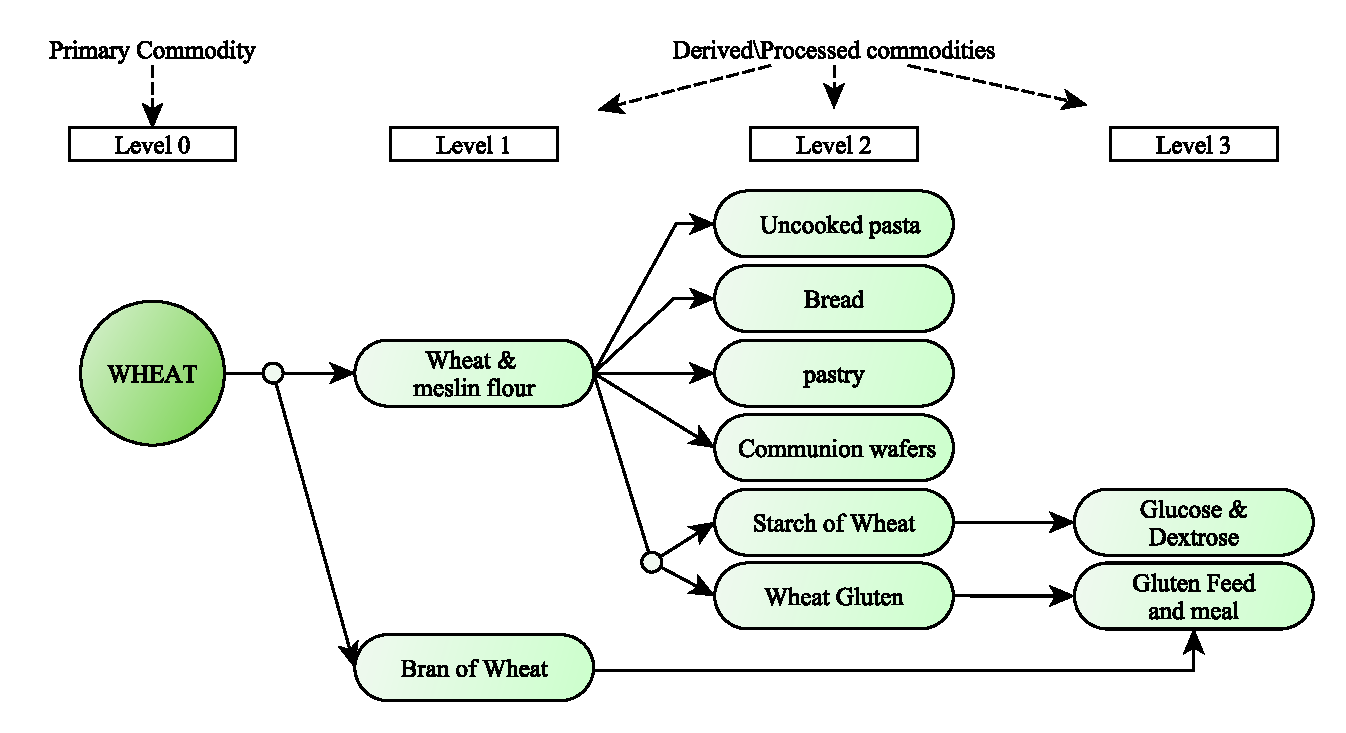
\includegraphics{images/02_WheatTree} 

}

\caption{\label{fig:f2}Commodity Tree for Wheat in China mainland 2014}\label{fig:f2}
\end{figure}

\begin{enumerate}
\def\labelenumi{\arabic{enumi}.}
\setcounter{enumi}{1}
\item
  Not all the countries use the same production processes, therefore the
  commodity trees are not the same across countries.
\item
  if a production process is active in a country, this is expressed
  trought the existence of a conversion factor called
  \textbf{\emph{extraction Rate}}. An Extraction rate (\(eR\))
  represents how much amount of the child commodity is produced from 1
  unit of parent commodity. It is expressed as a ratio of the processed
  product obtained from the processing of the parent/originating
  product.
\item
  Some child commodities can be produced starting from more that one
  parent commodity. A second conversion factor exists representing the
  amount of a child commodity that is produced from each parent
  ocmmodity. This conversion factor is called \textbf{\emph{Share}}.
  Shares represent the amount of the child commodity that is produced
  from the specified parent and are expressed as a ratio. Shares are
  generically defined as:
\end{enumerate}

\begin{quote}
\begin{equation}
\label{eq:sharesGen}
s_{cp} = \frac{availability_{p(c)}}{\sum \limits_{p=1}^A{availability_{p(c)}}}
\end{equation}
\end{quote}

\begin{quote}
where \(availability_{p(c)}\) is the availability of each parent \(p\)
of child \(c\) expressed in terms of \(c\) (as say in \emph{child
equivalent}). The availability \(availability_{p(c)}\) can be defined in
different ways during different steps of the overall process. In general
terms, it represents a difference between supply and utilizations, but
utilizations may be or not be all included in the calculation.
\end{quote}

Commodity trees are presented in tables like Table 1, which represents
the same example of Figure \ref{fig:f2}. In the table each production
process is represented in a separate row.

\begin{longtable}[]{@{}rlllll@{}}
\caption{Commodity Tree Wheat China Mainland, 2014}\tabularnewline
\toprule
Country & Year & ParentName & ChildName & eR & share\tabularnewline
\midrule
\endfirsthead
\toprule
Country & Year & ParentName & ChildName & eR & share\tabularnewline
\midrule
\endhead
China, Mainland & 2014 & Wheat & Wheat and meslin flo & 0.78 &
1.00\tabularnewline
China, Mainland & 2014 & Wheat & Bran of Wheat & 0.22 &
1.00\tabularnewline
China, Mainland & 2014 & Wheat and meslin flo & Uncooked pasta, not &
1.00 & 1.00\tabularnewline
China, Mainland & 2014 & Wheat and meslin flo & bread & 1.00 &
1.00\tabularnewline
China, Mainland & 2014 & Wheat and meslin flo & pastry & 1.00 &
1.00\tabularnewline
China, Mainland & 2014 & Wheat and meslin flo & Starch of Wheat & 0.75 &
1.00\tabularnewline
China, Mainland & 2014 & Wheat and meslin flo & Wheat Gluten & 0.08 &
1.00\tabularnewline
China, Mainland & 2014 & Wheat and meslin flo & Communion wafers, em &
1.00 & 1.00\tabularnewline
China, Mainland & 2014 & Starch of Wheat & Other Fructose and S & 1.00 &
1.00\tabularnewline
China, Mainland & 2014 & Wheat Gluten & Gluten Feed and Meal & 1.00 &
0.33\tabularnewline
China, Mainland & 2014 & Bran of Maize & Gluten Feed and Meal & 1.00 &
0.67\tabularnewline
\bottomrule
\end{longtable}

There are some concepts linked to the Commodity tree framework:

\begin{itemize}
\tightlist
\item
  \textbf{\emph{Proxi-Primary}} commodities. These are a set of
  commodities that are children of other commodities but, because they
  are important in representing the food availability of a country, are
  not aggregated to their primary commodities, but are kept separated.
  These commodities are \emph{cut} from the tree of the primary
  commodity/ies and, if they can be processed in other products, have
  their own commodity tree. The name \emph{proxi-primary} is assigned
  because they are considered as primary commodity in the Standarization
  process.
\item
  \textbf{\emph{No-Tree}} commodities. These are commodities that are
  primary commodities and are never processed in other products. As they
  are not involved in any production process, there is no tree
  associated to them. Notice that, even a commodity that is included in
  the commodity tree for one COuntry, might be a No-tree commodity for
  another countrt or another year, if no production processes have been
  activated for that specific commodity or year.
\end{itemize}

\section{Data Pull}\label{data-pull}

The process starts by considering the initial SUA for each commodity,
primary and derived, with the different variables of the equation (as
listed and briefly described in the previous section) filled with
figures as available from official or other sources and from imputation
and estimation method, when applied. In other words, the Process starts
by pulling figures inside a so-called \emph{SUA unbalanced}. In this
initial account food processing and RoU figures are not available
(because they, by default, will be measured during the process), whereas
the figures for all other variables have been already collected, imputed
and estimated through specific \emph{module} (Figure \ref{fig:f1}).

\begin{figure}[htbp]
\centering
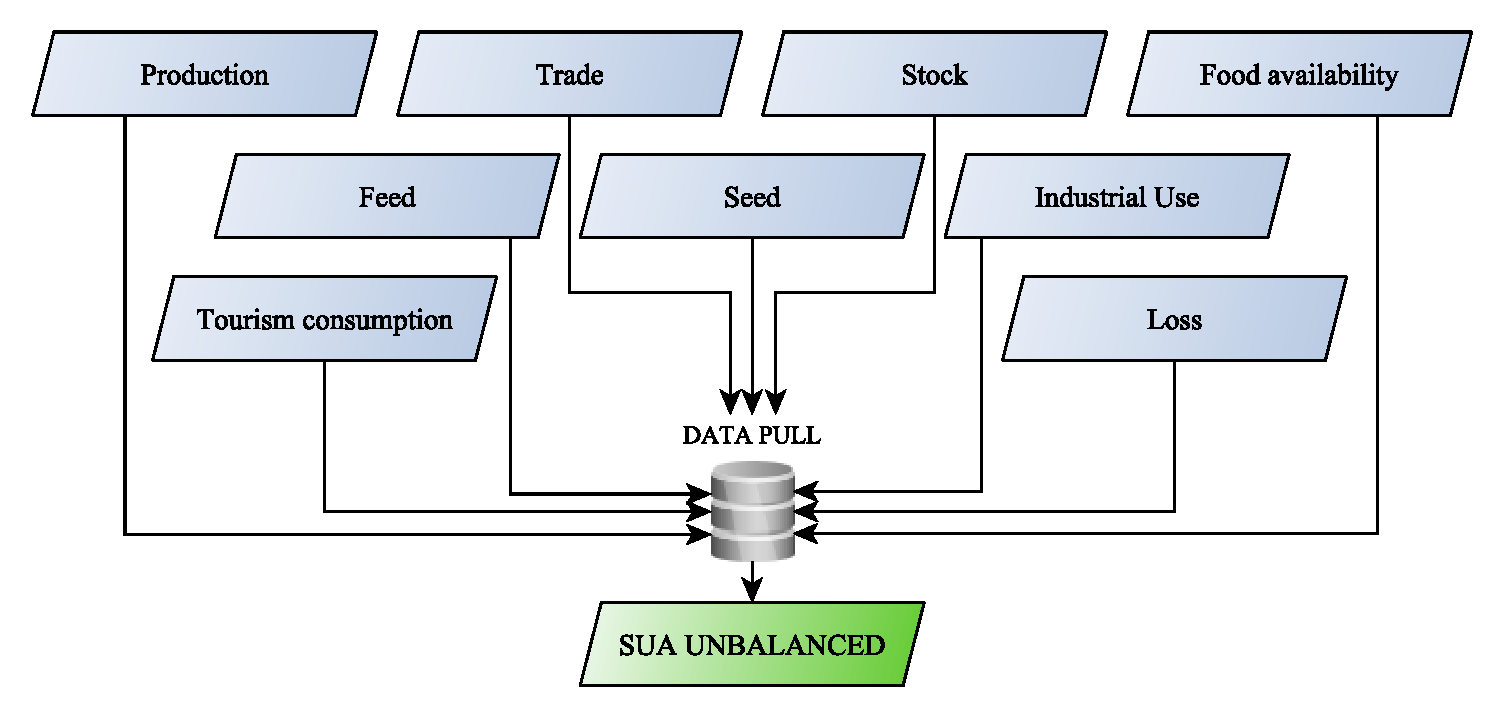
\includegraphics{images/01_pulldata.pdf}
\caption{\label{fig:f1}Data Pull from datasets containing data for each
separate variable}
\end{figure}

A module, in the FBS Framework, is an R-script, written by an
R-developer, for the execution of a set of operations (either data
import, manipulation, imputation or estimation) required for compiling
the time series of one variable. There is at least one module (there
might be more) for each variable of the FBS. Each module produces
figures that are collected in a dataset inside the \emph{Statistical
Working System (SWS)}\footnote{SWS is an internal Working System
  providing a platform for statisticians and statistical clers to
  collect, collate, validate and correct data. Moreover, the platfors
  supports the possibility of performing imputations of data based on
  statisticians' knowledge and development.}.Output data of a module may
become input data of another module, this creating a precise sequence
for the execution of a complete FBS. IN the present document we are
analyzing the workflow of the Standardization process as starts after
all the module have run and have produced reliable data or each
variable. The detailed description of the workflow for the execution of
al the module of the FBS is described in a separate document\footnote{{[}report
  the document when it will be available{]}}.

\section{the Initial Sua Unbalanced}\label{the-initial-sua-unbalanced}

After pulling all data, the process of compiling Food Balance Sheets is
a non-complete supply-utilization account. The non-completeness of the
SUAs is due to different reasons: first, as already said, some variables
are not collected, nor estimated before the process begins, second there
is the model for industrial use that does not impute or estimate data,
but just collects data from different sources, this opening the strong
possibility not to have values where they are supposed to exist and,
also, not guaranteeing consistency of data over time. Thirdly, modules
might, sometimes, fail in the imputation, because of the strong
complexity and structural diversity of the input data.

\begin{landscape}\begin{table}

\caption{\label{tab:t1}Unbalanced Sua table (Example China Mainland, Wheat 2014)}
\centering
\resizebox{\linewidth}{!}{\fontsize{18}{20}\selectfont
\begin{tabular}[t]{>{\raggedleft\arraybackslash}p{12em}|>{\raggedright\arraybackslash}p{6em}|>{\raggedright\arraybackslash}p{6em}|>{\raggedright\arraybackslash}p{6em}|>{\raggedright\arraybackslash}p{6em}|>{\raggedright\arraybackslash}p{6em}|>{\raggedright\arraybackslash}p{6em}|>{\raggedright\arraybackslash}p{6em}|>{\raggedright\arraybackslash}p{6em}|>{\raggedright\arraybackslash}p{6em}|>{\raggedright\arraybackslash}p{6em}|>{\raggedright\arraybackslash}p{6em}|>{\raggedright\arraybackslash}p{6em}}
\hline
\multicolumn{1}{r}{\textbf{itemName}} & \multicolumn{1}{c}{\textbf{P}} & \multicolumn{1}{c}{\textbf{I}} & \multicolumn{1}{c}{\textbf{X}} & \multicolumn{1}{c}{\textbf{DSt}} & \multicolumn{1}{c}{\textbf{Fo}} & \multicolumn{1}{c}{\textbf{FP}} & \multicolumn{1}{c}{\textbf{Fe}} & \multicolumn{1}{c}{\textbf{Se}} & \multicolumn{1}{c}{\textbf{T}} & \multicolumn{1}{c}{\textbf{IU}} & \multicolumn{1}{c}{\textbf{L}} & \multicolumn{1}{c}{\textbf{ROU}}\\
\hline
\em{Wheat} & \em{126,208,400} & \em{2,971,249} & \em{957} & \em{1,120,565} & \em{} & \em{-} & \em{29,181,617} & \em{4,277,567} & \em{} & \em{2,985,279} & \em{2,713,000} & \em{-}\\
\hline
Wheat and meslin flo & 70,500,000 & 33,055 & 188,674 &  & 67,300,000 & - &  &  & -17,345 &  &  & -\\
\hline
Mixes and doughs for &  & 6,497 & 38,072 &  & 0 & - & 0 &  & 0 &  &  & -\\
\hline
Other Fructose and S & 126,277 & 3,659 & 162,324 &  & 0 & - &  &  & 0 &  &  & -\\
\hline
Starch of Wheat & 239,816 & 11,035 & 40,311 &  &  & - & 172,196 &  &  & 7,919 &  & -\\
\hline
Wheat Gluten & 25,580 & 877 & 117,373 &  &  & - & 0 &  &  &  &  & -\\
\hline
Communion wafers & 13,263 & 8,796 & 5,822 &  & 16,241 & - &  &  & -4 &  &  & -\\
\hline
Uncooked pasta & 1,415,692 & 12,520 & 22,550 &  & 1,405,661 & - &  &  & -362 &  &  & -\\
\hline
Food Preparations of &  & 69,686 & 21,977 &  & 47,709 & - &  &  & -12 &  &  & -\\
\hline
Bran of Wheat & 21,414,279 & 156,359 & 2,200 &  & 16,500,000 & - & 4,827,244 &  & -4,252 &  &  & -\\
\hline
Gluten Feed and Meal & 793,740 & 160,231 & 529,333 &  &  & - &  &  &  &  &  & -\\
\hline
bread & 15,485 & 2,897 & 4,210 &  & 14,175 & - &  &  & -3 &  &  & -\\
\hline
pastry & 193,950 & 89,593 & 117,630 &  & 165,914 & - &  &  & -43 &  &  & -\\
\hline
\multicolumn{13}{l}{\textsuperscript{*} P=Production, I=Import, X=Export, DSt=Delta Stock, Fo=Food Availability, FP=FoodProcessing, Fe=Feed, Se=Seed, T=Tourism Consumption,}\\
\multicolumn{13}{l}{IU=IndustrialUse, L=Loss, ROU=Residual and other uses}\\
\end{tabular}}
\end{table}
\end{landscape}

Supply utilization accounts are typically organized into tables where
the SUA for the primary commodity is at the top, and the SUAs for all of
the products derived from that commodity follow (Table 2). Commodities
in the SUA table are in a parent-child relationship representing a real
commodity process. In the example of Table 2 the relationship between
commodities is the following:

\begin{itemize}
\tightlist
\item
  Maize is processed in flour, Bran and Breakfast Cereals,
\item
  Flour of maize is processed into Starch and Gluten, Wafers, pastry,
  bread and pasta
\item
  Starch is processed into Glucose and Dextrose,
\item
  Gluten and Bran are processed into some feed and meal,
\end{itemize}

All these relationships represent the \emph{Commodity tree} of wheat in
China in 2014. In particular, our example represents the commodity tree
of Wheat in China in 2014 and is displayed, in its graphical form, in
Figure \ref{fig:f2}.

There are unbalanced SUAs for all combinations of commodity
tree/country/year. These tables are the starting poin of the
\emph{Standardization and Balancing} process, which starts with the
``Filling'' of the missing figures in the SUAs.

\section{\texorpdfstring{The \emph{Sua
Filling}}{The Sua Filling}}\label{the-sua-filling}

\subsection*{Main rules and the
rationale}\label{main-rules-and-the-rationale}
\addcontentsline{toc}{subsection}{Main rules and the rationale}

The Standardization, i.e.~the conversion of the variables of any child
commodity in primary-equivalent commodity, requires all variables of the
SUAs to be filled (exept for ROU, which is a residual variable and is
imputed at the very last step of theprocess), ``all variables'' meaning
``all variables that are supposed to be filled''. Indeed, not all
variables have to exist for all commodities. Consider maize as an
example: if there is no figure of \emph{food availability} for maize,
that does not mean that there is a missing figure, because maize is
rarely used for human consumption directly. However, in some country
people do eat raw maize and, therefore, for those countries a food
figure is expected and, if missing, that has to be taken into account.

A simplifided workflow of \emph{Sua Filling} is reported in Figure
\ref{fig:f3}.

\begin{figure}[H]

{\centering \includegraphics[width=0.6\linewidth]{images/03_SuaFilling} 

}

\caption{\label{fig:f3}The Sua filling simplified workflow}\label{fig:f3}
\end{figure}

\emph{Food Processing} needs to be computed first, which does not come
from any module. For the food processing to be correclty computed, a
check on the other variables as to be performed, in order to be sure
that the food processing might be correclty imputed. In particular,
Production is checked first, as the \emph{Food Processing} figure of any
commodity is based on the production one. Then \emph{Food processing}
can be computed and, after that, other missing figures, if existing, are
filled.

This last step requires two major and not straightforward steps,
representing each a separate issue, for solving which, an algorithm has
been developed that responds to the following rationale and rules:

\begin{enumerate}
\def\labelenumi{\arabic{enumi}.}
\tightlist
\item
  \emph{Identify which are the missing values that have to be filled.}
\item
  \emph{Decide how to fill those missing values.}
\item
  \emph{Preserving reliability of sources of data}
\end{enumerate}

Not all the variables (supplies and utilizations) are to be filled:

\begin{itemize}
\tightlist
\item
  Trade (import and Export) data are shared with countries and published
  by FAO. Therefore these figures have a separate process of validation
  that makes them reliable enough not to be questioned during the
  standardization process.
\item
  Production figures of primary commodities are also published by FAO.
  As previously mentioned, production values can have various flags
  which assign different degrees of reliability to these figures. The
  \emph{sua filling} treats production figures accordingly to flags.
\item
  Stock figures are also not touched during the process of filling. This
  decision was taken because the standardization process works year by
  year, while \emph{stock variation} is a time-based variable that have
  to be always treated looking at the data over time. The cross year
  approach is incompatible with this characteristic. Any inconsistent or
  missing value for stock found would require to go back to the module
  imputing figures and check for possible errors. If no errors can be
  found, a manual correction would be required.
\end{itemize}

Information about the remaining variables, which are all utilizations,
is taken from FBSs and SUAs of past years. FBSs published with the
previous methodology and their corresponding SUAs can give information
about which are the utilizations supposed to be active for every single
commodity in each country.\\
Therefore, these information have to be given externally, as the process
is automated and there is non-human knowledge intervening in training
the machine that is performing the calculations. The previous
methodology used for compiling FBS made massive use of manual
interventions while the new methodology tries to avoid it, but taking
advantage of the work and effort of the country experts that compiled
the FBSs in the past. Past information are embedded in the new
methodology trought the use of the \emph{Utilization table} which helps
idenifying which variables have to be filled, commodity by commodity,
while the amount of the to be assiged to sigures is identified through a
set of rules, known as \emph{Sua filling}. This procedure makes use of
the imbalance between supply and utilization values for each commodity
and fills the figures that have been recognized as missing from the
\textbf{\emph{Utilization table}}. The filling procedure assigns figures
using an ad-hoc algorithm, called \textbf{\emph{Inverse Ranking}},
designed for dimensioning the figures in accordance with the importance
they had in the past FBSs, as suggested also from the \emph{Utilization
table} through ranks associated to each variable. As a consequence, all
the commodities entering the sua filling procedure are eventually
balanced.

Not all the commodities enter the process the same way. In particular, a
distinction is made between primary commodties and derived commodities:

\begin{itemize}
\tightlist
\item
  Primary commodities are normally the commodities for which more
  reliable figures are produced. Moreover, FAO often publish information
  about primary commodities, therefore values are not expected to be
  modifyed during a computational process.
\item
  Derived commodities are more affected by modifications during this
  process, according to the flag of each figure.
\end{itemize}

Therefore, the steps of \emph{Sua filling} process affect the SUA
differently from line to line. Figure \ref{fig:f4} shows the general
Workflow of the sua filling highlighting the distinction between primary
and derived commodities.

\begin{figure}

{\centering \includegraphics[width=0.65\linewidth]{images/04_SuaFilling2} 

}

\caption{\label{fig:f4}The Sua filling divesified workflow}\label{fig:f4}
\end{figure}

\subsection*{Step 1: Filling of production
figures}\label{step-1-filling-of-production-figures}
\addcontentsline{toc}{subsection}{Step 1: Filling of production figures}

Only Derived commodities are involved in this process. The sua filling
detect the Production figures that need to be filled or modified, by
looking at the following \emph{Imbalance}:

\begin{equation}
\label{eq:imbalance1}
Imb_{1} = P_{ijt} + I_{ijt} - X_{ijt}
\end{equation}

where \(Imb_{1}\) is the Imbalance and is enumerated because is
different from a second Imbalance that will enter into the process
later. Here:

\begin{itemize}
\tightlist
\item
  If \(Imb_{1} < 0\) there is no supply enough for the export and this
  is intepreted as the need for creating/incrementing the Production
  figure. The new production figure (\(P^*_{ijt}\)) is computed as:
\end{itemize}

\begin{equation}
\label{eq:imbalance1}
 P^*_{ijt} = P_{ijt} + Imb_{1}
\end{equation}

\begin{itemize}
\tightlist
\item
  If \(Imb_{1} >= 0\) there is enough supply and, therefore, no need for
  changing the production figure.
\end{itemize}

The reason for excluding other Variables from the computation of the
imbalance here is that, at this step of the process, Trade variables are
the most reliable and those for which, to the highest level of
probability, there are all the figures filled. In Table 3 \emph{Imb1} of
our example is reported. Notice that there are 3 rows with negative
values, but one of them is considered Primary ommodity. Indeed,
\emph{Mixes and dough for the preparation of baker's wares} is a
commodity never processed and, therefore, is considered primary
commodity and added to wheat in the FBS item \emph{Wheat and produts}.
Consequently production of only 2 commodity is changes, as shown in
Table 4.

\begin{landscape}\begin{table}

\caption{\label{tab:t2}Sua table with Imb1 (Example China Mainland, Wheat 2014)}
\centering
\resizebox{\linewidth}{!}{\fontsize{18}{20}\selectfont
\begin{tabular}[t]{>{\raggedleft\arraybackslash}p{12em}|l|>{\raggedright\arraybackslash\leavevmode\color{black}}p{6em}|>{\raggedright\arraybackslash\leavevmode\color{black}}p{6em}|>{\raggedright\arraybackslash\leavevmode\color{black}}p{6em}|>{\raggedright\arraybackslash\leavevmode\color{black}}p{6em}|>{\raggedright\arraybackslash\leavevmode\color{black}}p{6em}|>{\raggedright\arraybackslash\leavevmode\color{black}}p{6em}|>{\raggedright\arraybackslash\leavevmode\color{black}}p{6em}|>{\raggedright\arraybackslash\leavevmode\color{black}}p{6em}|>{\raggedright\arraybackslash\leavevmode\color{black}}p{6em}|>{\raggedright\arraybackslash\leavevmode\color{black}}p{6em}|>{\raggedright\arraybackslash\leavevmode\color{black}}p{6em}|>{\bfseries\em\leavevmode\color{red}}l}
\hline
\multicolumn{1}{r}{\textbf{itemName}} & \multicolumn{1}{c}{\textbf{P}} & \multicolumn{1}{c}{\textbf{I}} & \multicolumn{1}{c}{\textbf{X}} & \multicolumn{1}{c}{\textbf{DSt}} & \multicolumn{1}{c}{\textbf{Fo}} & \multicolumn{1}{c}{\textbf{FP}} & \multicolumn{1}{c}{\textbf{Fe}} & \multicolumn{1}{c}{\textbf{Se}} & \multicolumn{1}{c}{\textbf{T}} & \multicolumn{1}{c}{\textbf{IU}} & \multicolumn{1}{c}{\textbf{L}} & \multicolumn{1}{c}{\textbf{ROU}} & \multicolumn{1}{c}{\textbf{Imb1}}\\
\hline
Wheat & 126,208,400 & 2,971,249 & 957 & 1,120,565 &  & - & 29,181,617 & 4,277,567 &  & 2,985,279 & 2,713,000 & - & 129,178,692\\
\hline
Wheat and meslin flo & 70,500,000 & 33,055 & 188,674 &  & 67,300,000 & - &  &  & -17,345 &  &  & - & 70,344,381\\
\hline
Mixes and doughs for &  & 6,497 & 38,072 &  & 0 & - & 0 &  & 0 &  &  & - & -31,575\\
\hline
Other Fructose and S & 126,277 & 3,659 & 162,324 &  & 0 & - &  &  & 0 &  &  & - & -32,388\\
\hline
Starch of Wheat & 239,816 & 11,035 & 40,311 &  &  & - & 172,196 &  &  & 7,919 &  & - & 210,541\\
\hline
Wheat Gluten & 25,580 & 877 & 117,373 &  &  & - & 0 &  &  &  &  & - & -90,916\\
\hline
Communion wafers & 13,263 & 8,796 & 5,822 &  & 16,241 & - &  &  & -4 &  &  & - & 16,237\\
\hline
Uncooked pasta & 1,415,692 & 12,520 & 22,550 &  & 1,405,661 & - &  &  & -362 &  &  & - & 1,405,661\\
\hline
Food Preparations of &  & 69,686 & 21,977 &  & 47,709 & - &  &  & -12 &  &  & - & 47,709\\
\hline
Bran of Wheat & 21,414,279 & 156,359 & 2,200 &  & 16,500,000 & - & 4,827,244 &  & -4,252 &  &  & - & 21,568,438\\
\hline
Gluten Feed and Meal & 793,740 & 160,231 & 529,333 &  &  & - &  &  &  &  &  & - & 424,638\\
\hline
bread & 15,485 & 2,897 & 4,210 &  & 14,175 & - &  &  & -3 &  &  & - & 14,172\\
\hline
pastry & 193,950 & 89,593 & 117,630 &  & 165,914 & - &  &  & -43 &  &  & - & 165,914\\
\hline
\multicolumn{14}{l}{\textsuperscript{*} P=Production, I=Import, X=Export, DSt=Delta Stock, Fo=Food Availability, FP=FoodProcessing, Fe=Feed, Se=Seed, T=Tourism Consumption, IU=IndustrialUse,}\\
\multicolumn{14}{l}{L=Loss, ROU=Residual and other uses}\\
\end{tabular}}
\end{table}
\end{landscape}

\begin{landscape}\begin{table}

\caption{\label{tab:t3}Sua table with Production filled/incremented (Example China Mainland, Wheat 2014)}
\centering
\resizebox{\linewidth}{!}{\fontsize{18}{20}\selectfont
\begin{tabular}[t]{>{\raggedleft\arraybackslash}p{12em}|l|>{\raggedright\arraybackslash\leavevmode\color{black}}p{6em}|>{\raggedright\arraybackslash\leavevmode\color{black}}p{6em}|>{\raggedright\arraybackslash\leavevmode\color{black}}p{6em}|>{\raggedright\arraybackslash\leavevmode\color{black}}p{6em}|>{\raggedright\arraybackslash\leavevmode\color{black}}p{6em}|>{\raggedright\arraybackslash\leavevmode\color{black}}p{6em}|>{\raggedright\arraybackslash\leavevmode\color{black}}p{6em}|>{\raggedright\arraybackslash\leavevmode\color{black}}p{6em}|>{\raggedright\arraybackslash\leavevmode\color{black}}p{6em}|>{\raggedright\arraybackslash\leavevmode\color{black}}p{6em}|>{\raggedright\arraybackslash\leavevmode\color{black}}p{6em}|>{\raggedright\arraybackslash\leavevmode\color{black}}p{6em}}
\hline
\multicolumn{1}{r}{\textbf{itemName}} & \multicolumn{1}{c}{\textbf{P}} & \multicolumn{1}{c}{\textbf{I}} & \multicolumn{1}{c}{\textbf{X}} & \multicolumn{1}{c}{\textbf{DSt}} & \multicolumn{1}{c}{\textbf{Fo}} & \multicolumn{1}{c}{\textbf{FP}} & \multicolumn{1}{c}{\textbf{Fe}} & \multicolumn{1}{c}{\textbf{Se}} & \multicolumn{1}{c}{\textbf{T}} & \multicolumn{1}{c}{\textbf{IU}} & \multicolumn{1}{c}{\textbf{L}} & \multicolumn{1}{c}{\textbf{ROU}} & \multicolumn{1}{c}{\textbf{Imb1}}\\
\hline
Wheat & 126,208,400 & 2,971,249 & 957 & 1,120,565 &  & - & 29,181,617 & 4,277,567 &  & 2,985,279 & 2,713,000 & - & 129,178,692\\
\hline
Wheat and meslin flo & 70,500,000 & 33,055 & 188,674 &  & 67,300,000 & - &  &  & -17,345 &  &  & - & 70,344,381\\
\hline
Mixes and doughs for &  & 6,497 & 38,072 &  & 0 & - & 0 &  & 0 &  &  & - & -31,575\\
\hline
\textcolor{red}{\em{\textbf{Other Fructose and S}}} & \textcolor{red}{\em{\textbf{**158,665**}}} & \textcolor{red}{\em{\textbf{3,659}}} & \textcolor{red}{\em{\textbf{162,324}}} & \textcolor{red}{\em{\textbf{}}} & \textcolor{red}{\em{\textbf{0}}} & \textcolor{red}{\em{\textbf{-}}} & \textcolor{red}{\em{\textbf{}}} & \textcolor{red}{\em{\textbf{}}} & \textcolor{red}{\em{\textbf{0}}} & \textcolor{red}{\em{\textbf{}}} & \textcolor{red}{\em{\textbf{}}} & \textcolor{red}{\em{\textbf{-}}} & \textcolor{red}{\em{\textbf{0}}}\\
\hline
Starch of Wheat & 239,816 & 11,035 & 40,311 &  &  & - & 172,196 &  &  & 7,919 &  & - & 210,541\\
\hline
\textcolor{red}{\em{\textbf{Wheat Gluten}}} & \textcolor{red}{\em{\textbf{**116,496**}}} & \textcolor{red}{\em{\textbf{877}}} & \textcolor{red}{\em{\textbf{117,373}}} & \textcolor{red}{\em{\textbf{}}} & \textcolor{red}{\em{\textbf{}}} & \textcolor{red}{\em{\textbf{-}}} & \textcolor{red}{\em{\textbf{0}}} & \textcolor{red}{\em{\textbf{}}} & \textcolor{red}{\em{\textbf{}}} & \textcolor{red}{\em{\textbf{}}} & \textcolor{red}{\em{\textbf{}}} & \textcolor{red}{\em{\textbf{-}}} & \textcolor{red}{\em{\textbf{0}}}\\
\hline
Communion wafers & 13,263 & 8,796 & 5,822 &  & 16,241 & - &  &  & -4 &  &  & - & 16,237\\
\hline
Uncooked pasta & 1,415,692 & 12,520 & 22,550 &  & 1,405,661 & - &  &  & -362 &  &  & - & 1,405,661\\
\hline
Food Preparations of &  & 69,686 & 21,977 &  & 47,709 & - &  &  & -12 &  &  & - & 47,709\\
\hline
Bran of Wheat & 21,414,279 & 156,359 & 2,200 &  & 16,500,000 & - & 4,827,244 &  & -4,252 &  &  & - & 21,568,438\\
\hline
Gluten Feed and Meal & 793,740 & 160,231 & 529,333 &  &  & - &  &  &  &  &  & - & 424,638\\
\hline
bread & 15,485 & 2,897 & 4,210 &  & 14,175 & - &  &  & -3 &  &  & - & 14,172\\
\hline
pastry & 193,950 & 89,593 & 117,630 &  & 165,914 & - &  &  & -43 &  &  & - & 165,914\\
\hline
\multicolumn{14}{l}{\textsuperscript{*} P=Production, I=Import, X=Export, DSt=Delta Stock, Fo=Food Availability, FP=FoodProcessing, Fe=Feed, Se=Seed, T=Tourism Consumption, IU=IndustrialUse,}\\
\multicolumn{14}{l}{L=Loss, ROU=Residual and other uses}\\
\end{tabular}}
\end{table}
\end{landscape}

\subsection*{Step 2: Filling of food
processing}\label{step-2-filling-of-food-processing}
\addcontentsline{toc}{subsection}{Step 2: Filling of food processing}

When Production has been checked, created or incremented, \emph{Food
Processing} can be calculated. Food processing is the amount of the
supply of a commodity processed into derived commodities. \emph{Food
processing} is calculated for all the parent commodities as sum of the
food processing of all the possible derived commodities. For example,
Wheat in China is processed into Flour of Wheat, Bran of Wheatand
Breakfast Cereals: Flour and Bran are produced during the same
production process (they are called \emph{co-products} or
\emph{by-products}), therefore the same amount of wheat is used for
producing all of them, Breakfast Cereals comes from a separate
production process instead. Therefore, \emph{Food processing} of Wheat
is given as sum of the amount of wheat's supply used for priducing Flour
and Bran + The amount used for producing Breakfast Cereals. Calculation
of Food processing happens by level, then after having calculated the
amount for wheat, the amount of supply of flour of wheat used for
producing Starch, Gluten, bread and the other derived of wheat flour
becomes the \emph{Food processing} of flour of Wheat and so on, for any
subsequent level.

The formula for calculating \(FP\) is based on the production of the
child product:

\begin{equation}
\label{eq:Food Processing}
FP_{p_{ijt}} = \sum \limits_{c=1}^C\biggl(\frac{P_{c_{ijt}}}{eR_{p\to c}}\biggr)\times s_{cp}\times w_{c}
\end{equation}

where:

\begin{itemize}
\tightlist
\item
  \(FP_{p_{ijt}}\) is \emph{Food processing} of the generic parent
  \(p\).
\item
  \(c = 1,2,3...C\) are the \(C\) children \(c\) of parent \(p\).
\item
  \(P_{c_{ijt}}\) is the Production of Child \(c\).
\item
  \(eR_{p\to c}\) is the \emph{extraction Rate} from parent \(p\) to
  child \(c\).
\item
  \(s_{cp}\) is the \emph{share} of child \(c\) from parent \(p\).
  Shares here are defined as:
\end{itemize}

\begin{quote}
\begin{equation}
\label{eq:shares}
s_{cp} = \frac{availability1_{p(c)}}{\sum \limits_{p=1}^A{availability1_{p(c)}}}
\end{equation}
\end{quote}

\begin{quote}
where \(availability1_{p(c)}\) is the availability of each parent \(p\)
of child \(c\) expressed in terms of \(c\) (as say in \emph{child
equivalent}). Is is enumerated as \(1\) because a slighlty different
availability will be found in a following step:
\end{quote}

\begin{quote}
\begin{quote}
\begin{equation}
\label{eq:availability 1}
availability1_{p(c)} = (P_{p_{ijt}} + I_{p_{ijt}})\times eR_{p\to c}
\end{equation}
\end{quote}
\end{quote}

\begin{itemize}
\tightlist
\item
  \(w_{c}\) is the \emph{weight} of child \(c\). This parameter is used
  for identifying and treating co-product. Indeed, if the production of
  two or more co-prodiucts is used for producing \emph{Food processing}
  of the parent commodity producing them, the result would be a Food
  processing twice the size of what it should be. This would happen
  because the two co-products are produced during the same process, in
  other words, fromt he same amount of the parent commodity. For this to
  be taken into account, a weight is used, which is 1 for the commodity
  that have to be considered for determining Food processing of parent
  commodity and 0 for the child commodity that are co-products (equation
  \ref{eq:weight}). Please notice that, the co-products are still
  important in the standardization, because they contribute in the
  creation of the calories availability of the country, therefore, these
  commodities (Also called \emph{zero weight} commodities) are
  multiplied by 0 only when quantities are treated, they will instead be
  considered when calories will be taken into account:
\end{itemize}

\begin{quote}
\begin{quote}
\begin{equation}
\label{eq:weight}
\begin{cases}
w_{c} = 1      & \quad \text{if boht quantity and calories have to be standardized} \\
w_{c} = 0      & \quad \text{if only calories have to be standardized}
\end{cases}
\end{equation}
\end{quote}
\end{quote}

The following Table reports the commodity tree of the wheat/China
example with the extracolumn reporting the \emph{weight} of each
child-commodity.

\begin{longtable}[]{@{}rllllll@{}}
\caption{Commodity Tree Wheat China Mainland, 2014 with
weights}\tabularnewline
\toprule
Country & Year & ParentName & ChildName & eR & share &
weight\tabularnewline
\midrule
\endfirsthead
\toprule
Country & Year & ParentName & ChildName & eR & share &
weight\tabularnewline
\midrule
\endhead
China, Mainland & 2014 & Wheat & Wheat and meslin flo & 0.78 & 1.00 &
1\tabularnewline
China, Mainland & 2014 & Wheat & Bran of Wheat & 0.22 & 1.00 &
0\tabularnewline
China, Mainland & 2014 & Wheat and meslin flo & Uncooked pasta, not &
1.00 & 1.00 & 1\tabularnewline
China, Mainland & 2014 & Wheat and meslin flo & bread & 1.00 & 1.00 &
1\tabularnewline
China, Mainland & 2014 & Wheat and meslin flo & pastry & 1.00 & 1.00 &
1\tabularnewline
China, Mainland & 2014 & Wheat and meslin flo & Starch of Wheat & 0.75 &
1.00 & 1\tabularnewline
China, Mainland & 2014 & Wheat and meslin flo & Wheat Gluten & 0.08 &
1.00 & 0\tabularnewline
China, Mainland & 2014 & Wheat and meslin flo & Communion wafers, em &
1.00 & 1.00 & 1\tabularnewline
China, Mainland & 2014 & Starch of Wheat & Other Fructose and S & 1.00 &
1.00 & 1\tabularnewline
China, Mainland & 2014 & Wheat Gluten & Gluten Feed and Meal & 1.00 &
0.33 & 0\tabularnewline
China, Mainland & 2014 & Bran of Maize & Gluten Feed and Meal & 1.00 &
0.67 & 0\tabularnewline
\bottomrule
\end{longtable}

Shares lower than \(1\) mean that the child commodity might be produced
also from other parents and, therefore, the reported ratio represents
the ratio of that commodity that is produced from the reported parent.
For example, \emph{Gluten Feed and Meal} is produced from \emph{Wheat
Gluten} and from \emph{Bran of maize}. The sum of the shares associated
to this child (\(0.33\) and \(0.67\)) is equal to \(1\).

Table 6 shows the SUA table after the two steps just described. Notice
that, in the specific example, there was no need for the
creation/incrementation of Production on any derived commodity because
\(Imb1\) is positive for all commodities.

From Table 5 and Table 6 here is, as example, the computation of
\emph{Food processing} of Wheat,Flour of wheat and Starch of wheat:

\begin{equation}
\begin{multlined}
\label{eq:wheatFP}
FP_{wheat_{2014}} = \left(70,500,000/0.78\right)\times 1\times 1 +\left(21,414,729/0.8\right)\times 1\times 0 = 90,384,615
\end{multlined}
\end{equation}

\begin{equation}
\begin{multlined}
\label{eq:flourFP}
FP_{flourW_{2014}} = \left(1,415,692/1\right)\times 1\times 1 +\left(15,486/1\right)\times 1\times 1 
+\left(193,950/1\right)\times 1\times 1
+\\
\left(239,816/0.75\right)\times 1\times 1 +
\left(116,496/1\right)\times 1\times 0 +\left(13,263/1\right)\times 1\times 1= 1,958,146
\end{multlined}
\end{equation}

\begin{equation}
\begin{multlined}
\label{eq:starchFP}
FP_{starchW_{2014}} = \left(158,665/1\right)\times 1\times 1 +\left(21,414,729/0.8\right)\times 1\times 0 = 158,665
\end{multlined}
\end{equation}

\begin{landscape}\begin{table}

\caption{\label{tab:t5}Sua table with Food Processing filled (Example China Mainland, Wheat 2014)}
\centering
\resizebox{\linewidth}{!}{\fontsize{18}{20}\selectfont
\begin{tabular}[t]{>{\raggedleft\arraybackslash}p{12em}|>{\raggedright\arraybackslash}p{6em}|>{\raggedright\arraybackslash}p{6em}|>{\raggedright\arraybackslash}p{6em}|>{\raggedright\arraybackslash}p{6em}|>{\raggedright\arraybackslash}p{6em}|>{\bfseries\em\leavevmode\color{red}}l|>{\raggedright\arraybackslash}p{6em}|>{\raggedright\arraybackslash}p{6em}|>{\raggedright\arraybackslash}p{6em}|>{\raggedright\arraybackslash}p{6em}|>{\raggedright\arraybackslash}p{6em}|>{\raggedright\arraybackslash}p{6em}}
\hline
\multicolumn{1}{r}{\textbf{itemName}} & \multicolumn{1}{c}{\textbf{P}} & \multicolumn{1}{c}{\textbf{I}} & \multicolumn{1}{c}{\textbf{X}} & \multicolumn{1}{c}{\textbf{DSt}} & \multicolumn{1}{c}{\textbf{Fo}} & \multicolumn{1}{c}{\textbf{FP}} & \multicolumn{1}{c}{\textbf{Fe}} & \multicolumn{1}{c}{\textbf{Se}} & \multicolumn{1}{c}{\textbf{T}} & \multicolumn{1}{c}{\textbf{IU}} & \multicolumn{1}{c}{\textbf{L}} & \multicolumn{1}{c}{\textbf{ROU}}\\
\hline
Wheat & 126,208,400 & 2,971,249 & 957 & 1,120,565 &  & **90,384,615** & 29,181,617 & 4,277,567 &  & 2,985,279 & 2,713,000 & -\\
\hline
Wheat and meslin flo & 70,500,000 & 33,055 & 188,674 &  & 67,300,000 & **1,958,146** &  &  & -17,345 &  &  & -\\
\hline
Mixes and doughs for &  & 6,497 & 38,072 &  & 0 &  & 0 &  & 0 &  &  & -\\
\hline
Other Fructose and S & 158,665 & 3,659 & 162,324 &  & 0 &  &  &  & 0 &  &  & -\\
\hline
Starch of Wheat & 239,816 & 11,035 & 40,311 &  &  & **158,664** & 172,196 &  &  & 7,919 &  & -\\
\hline
Wheat Gluten & 116,496 & 877 & 117,373 &  &  & **0** & 0 &  &  &  &  & -\\
\hline
Communion wafers & 13,263 & 8,796 & 5,822 &  & 16,241 &  &  &  & -4 &  &  & -\\
\hline
Uncooked pasta & 1,415,692 & 12,520 & 22,550 &  & 1,405,661 &  &  &  & -362 &  &  & -\\
\hline
Food Preparations of &  & 69,686 & 21,977 &  & 47,709 &  &  &  & -12 &  &  & -\\
\hline
Bran of Wheat & 21,414,279 & 156,359 & 2,200 &  & 16,500,000 &  & 4,827,244 &  & -4,252 &  &  & -\\
\hline
Gluten Feed and Meal & 793,740 & 160,231 & 529,333 &  &  &  &  &  &  &  &  & -\\
\hline
bread & 15,485 & 2,897 & 4,210 &  & 14,175 &  &  &  & -3 &  &  & -\\
\hline
pastry & 193,950 & 89,593 & 117,630 &  & 165,914 &  &  &  & -43 &  &  & -\\
\hline
\multicolumn{13}{l}{\textsuperscript{*} P=Production, I=Import, X=Export, DSt=Delta Stock, Fo=Food Availability, FP=FoodProcessing, Fe=Feed, Se=Seed, T=Tourism Consumption, IU=IndustrialUse,}\\
\multicolumn{13}{l}{L=Loss, ROU=Residual and other uses}\\
\end{tabular}}
\end{table}
\end{landscape}

\subsection*{Step 3: Filling of other missing
utilizations}\label{step-3-filling-of-other-missing-utilizations}
\addcontentsline{toc}{subsection}{Step 3: Filling of other missing
utilizations}

After \emph{Food processing} figures have been computed, the other
variables have to be checked and either filled, increased or decreased.
Only derived commodities enter this step. Primary commodities are
excluded because for these commodities, the figures are normally more
reliable and complete and, very often protected. Only the final
balancing may affect Primary commodity figures. This step is based on
the value of the following Imbalance:

\begin{equation}
\label{eq:imbalance2}
Imb_{2} = P_{ijt} + I_{ijt} - X_{ijt} - \Delta St_{ijt} - Fo_{ijt} - Fe_{ijt} - Lo_{ijt} - Se_{ijt} - IU_{ijt} - T_{ijt}
\end{equation}

Table 7 reports \(Imb2\) for all the lines of the SUAs of our example.

Three different scenarios con be found (Figure 5):

\begin{figure}

{\centering 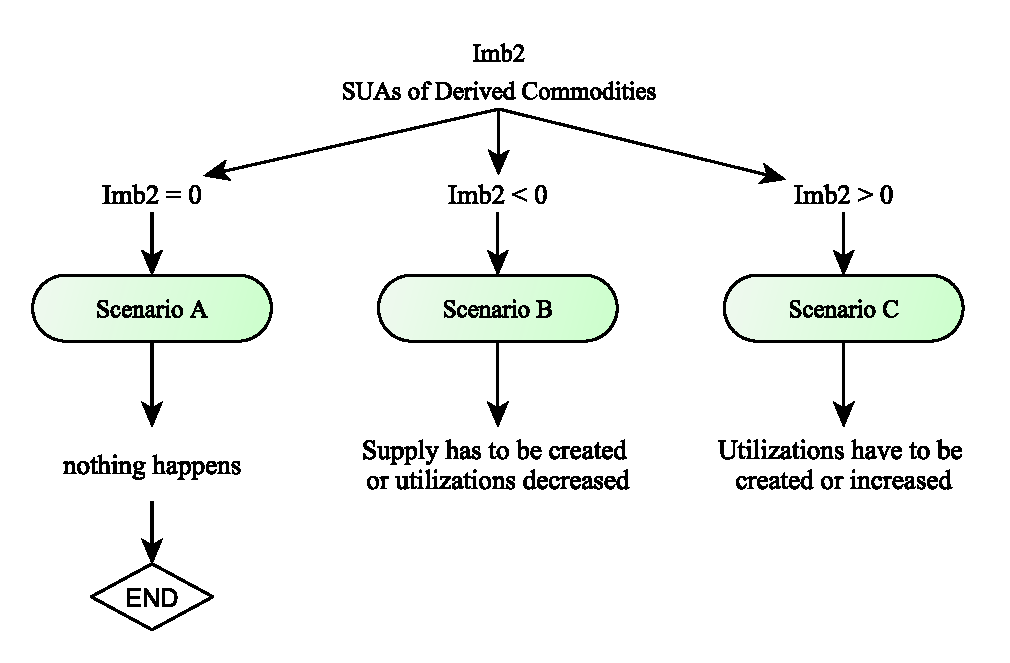
\includegraphics[width=0.8\linewidth]{images/05_ScenariosFilling} 

}

\caption{\label{fig:f5}Scenarios of the sua filling}\label{fig:f5}
\end{figure}

\begin{landscape}\begin{table}

\caption{\label{tab:t6}Sua table with Imb2 (Example China Mainland, Wheat 2014)}
\centering
\resizebox{\linewidth}{!}{\fontsize{18}{20}\selectfont
\begin{tabular}[t]{>{\raggedleft\arraybackslash}p{10em}|l|>{\raggedright\arraybackslash\leavevmode\color{black}}p{6em}|>{\raggedright\arraybackslash\leavevmode\color{black}}p{6em}|>{\raggedright\arraybackslash\leavevmode\color{black}}p{6em}|>{\raggedright\arraybackslash\leavevmode\color{black}}p{6em}|>{\raggedright\arraybackslash\leavevmode\color{black}}p{6em}|>{\raggedright\arraybackslash\leavevmode\color{black}}p{6em}|>{\raggedright\arraybackslash\leavevmode\color{black}}p{6em}|>{\raggedright\arraybackslash\leavevmode\color{black}}p{6em}|>{\raggedright\arraybackslash\leavevmode\color{black}}p{6em}|>{\raggedright\arraybackslash\leavevmode\color{black}}p{6em}|>{\raggedright\arraybackslash\leavevmode\color{black}}p{6em}|>{\bfseries\em\leavevmode\color{red}}l}
\hline
\multicolumn{1}{r}{\textbf{itemName}} & \multicolumn{1}{c}{\textbf{P}} & \multicolumn{1}{c}{\textbf{I}} & \multicolumn{1}{c}{\textbf{X}} & \multicolumn{1}{c}{\textbf{DSt}} & \multicolumn{1}{c}{\textbf{Fo}} & \multicolumn{1}{c}{\textbf{FP}} & \multicolumn{1}{c}{\textbf{Fe}} & \multicolumn{1}{c}{\textbf{Se}} & \multicolumn{1}{c}{\textbf{T}} & \multicolumn{1}{c}{\textbf{IU}} & \multicolumn{1}{c}{\textbf{L}} & \multicolumn{1}{c}{\textbf{ROU}} & \multicolumn{1}{c}{\textbf{Imb2}}\\
\hline
Wheat & 126,208,400 & 2,971,249 & 957 & 1,120,565 &  & 90,384,615 & 29,181,617 & 4,277,567 &  & 2,985,279 & 2,713,000 & - & -1,483,951\\
\hline
Wheat and meslin flo & 70,500,000 & 33,055 & 188,674 &  & 67,300,000 & 1,958,146 &  &  & -17,345 &  &  & - & 1,103,580\\
\hline
Mixes and doughs for &  & 6,497 & 38,072 &  & 0 &  & 0 &  & 0 &  &  & - & -31,575\\
\hline
Other Fructose and S & 158,665 & 3,659 & 162,324 &  & 0 &  &  &  & 0 &  &  & - & 0\\
\hline
Starch of Wheat & 239,816 & 11,035 & 40,311 &  &  & 158,664 & 172,196 &  &  & 7,919 &  & - & -128,239\\
\hline
Wheat Gluten & 116,496 & 877 & 117,373 &  &  & 0 & 0 &  &  &  &  & - & 0\\
\hline
Communion wafers & 13,263 & 8,796 & 5,822 &  & 16,241 &  &  &  & -4 &  &  & - & 0\\
\hline
Uncooked pasta & 1,415,692 & 12,520 & 22,550 &  & 1,405,661 &  &  &  & -362 &  &  & - & 363\\
\hline
Food Preparations of &  & 69,686 & 21,977 &  & 47,709 &  &  &  & -12 &  &  & - & 12\\
\hline
Bran of Wheat & 21,414,279 & 156,359 & 2,200 &  & 16,500,000 &  & 4,827,244 &  & -4,252 &  &  & - & 245,447\\
\hline
Gluten Feed and Meal & 793,740 & 160,231 & 529,333 &  &  &  &  &  &  &  &  & - & 424,638\\
\hline
bread & 15,485 & 2,897 & 4,210 &  & 14,175 &  &  &  & -3 &  &  & - & 0\\
\hline
pastry & 193,950 & 89,593 & 117,630 &  & 165,914 &  &  &  & -43 &  &  & - & 42\\
\hline
\multicolumn{14}{l}{\textsuperscript{*} P=Production, I=Import, X=Export, DSt=Delta Stock, Fo=Food Availability, FP=FoodProcessing, Fe=Feed, Se=Seed, T=Tourism Consumption, IU=IndustrialUse, L=Loss,}\\
\multicolumn{14}{l}{ROU=Residual and other uses}\\
\end{tabular}}
\end{table}
\end{landscape}

Please notice that, besides export and stock Variations, that are
excluded from this step for the reasons previously explained, also Food
Procesisng is excluded from the next steps, because \(FP\) is related to
the production figures of the children and to modify it, would detach
this very important parent-children link.

\subsubsection*{\texorpdfstring{\emph{Imbalance = 0 (Scenario
A)}}{Imbalance = 0 (Scenario A)}}\label{imbalance-0-scenario-a}
\addcontentsline{toc}{subsubsection}{\emph{Imbalance = 0 (Scenario A)}}

In this scenario the Imbalance is null, this meaning that there is
enought supply for the existing utilizations. In This case the SUA line
is balanced and nothig happens for the commodity. In Table 7 this is the
case of \emph{Other Fructose and syrup} and \emph{wheat Gluten}.

\subsubsection*{\texorpdfstring{\emph{Imbalance \textless{} 0 (Scenario
B)}}{Imbalance \textless{} 0 (Scenario B)}}\label{imbalance-0-scenario-b}
\addcontentsline{toc}{subsubsection}{\emph{Imbalance \textless{} 0
(Scenario B)}}

If this happens, it means that there is not enough supply for the
commodity to be used in the way the SUA figures suggest. First of all it
has to be rembered that, as said in a previous section, trade figures
are never changed during the filling process, this meaning that, if
there is a need for interveening on supply, only production figures
might be taken into account. In this case, as shown in Figure
\ref{fig:f6} a distinction as to be made as of the Production figure is
protected or not.

\begin{itemize}
\tightlist
\item
  If Production figure is not protected, it is interpreted as if there
  was not enough information for producing a correct production number,
  therefore, this figure is changed, i.e.~created, if missing, or
  incremented.
\item
  If Production figure is protected, it should never be touched,
  therefore the algoritm tries to solve the eccess of utilization by
  reducing all the existing utilizations by 30\% (except
  Exports\footnote{Stock is changed in this case, because this is just a
    proportional reduction of values and does not need a time series
    analysis}). If this is enough to cover the Utilization, the
  balancing line for that commodity is balanced and the process can go
  to the next step. After the reduction by 30\%, the imbalance \(Imb2\)
  is recalculated and it can give two different results:
\end{itemize}

\begin{quote}
-- If this imbalance is still negative a warning is given that tells
that there is an unsolvable problem and that all figures have to be
checked because either the production protected figure is wrong, or the
Trade or some utilization have to be changed.
\end{quote}

\begin{quote}
-- If the imbalance becomes positive, the line falls into the Scenario C
that will be explained shortly.
\end{quote}

\emph{Starch of Wheat} belongs to this very last case. Indeed, it has a
negative Imbalance therefore its utilizations (except those utilizations
that are completely excluded from this process) are reduced by 30\% of
their values (see Table 8). After that happens, the Imb2 is recalculated
and it is still negative, equal to \(74,204\) (this value is not
reported in the table). In the following step, as the production is not
protected, the new value of production is equal to:

\begin{equation}
\label{eq:prod}
P_{StarchW} = 239,816 + 74,204 = 314,020
\end{equation}

Remember that the commodity \emph{Mixes and dough for the preparation of
baker's wares}is considered here as a primary commodity, therefore it
will not balanced even if it has a negative imbalance.

\begin{figure}

{\centering 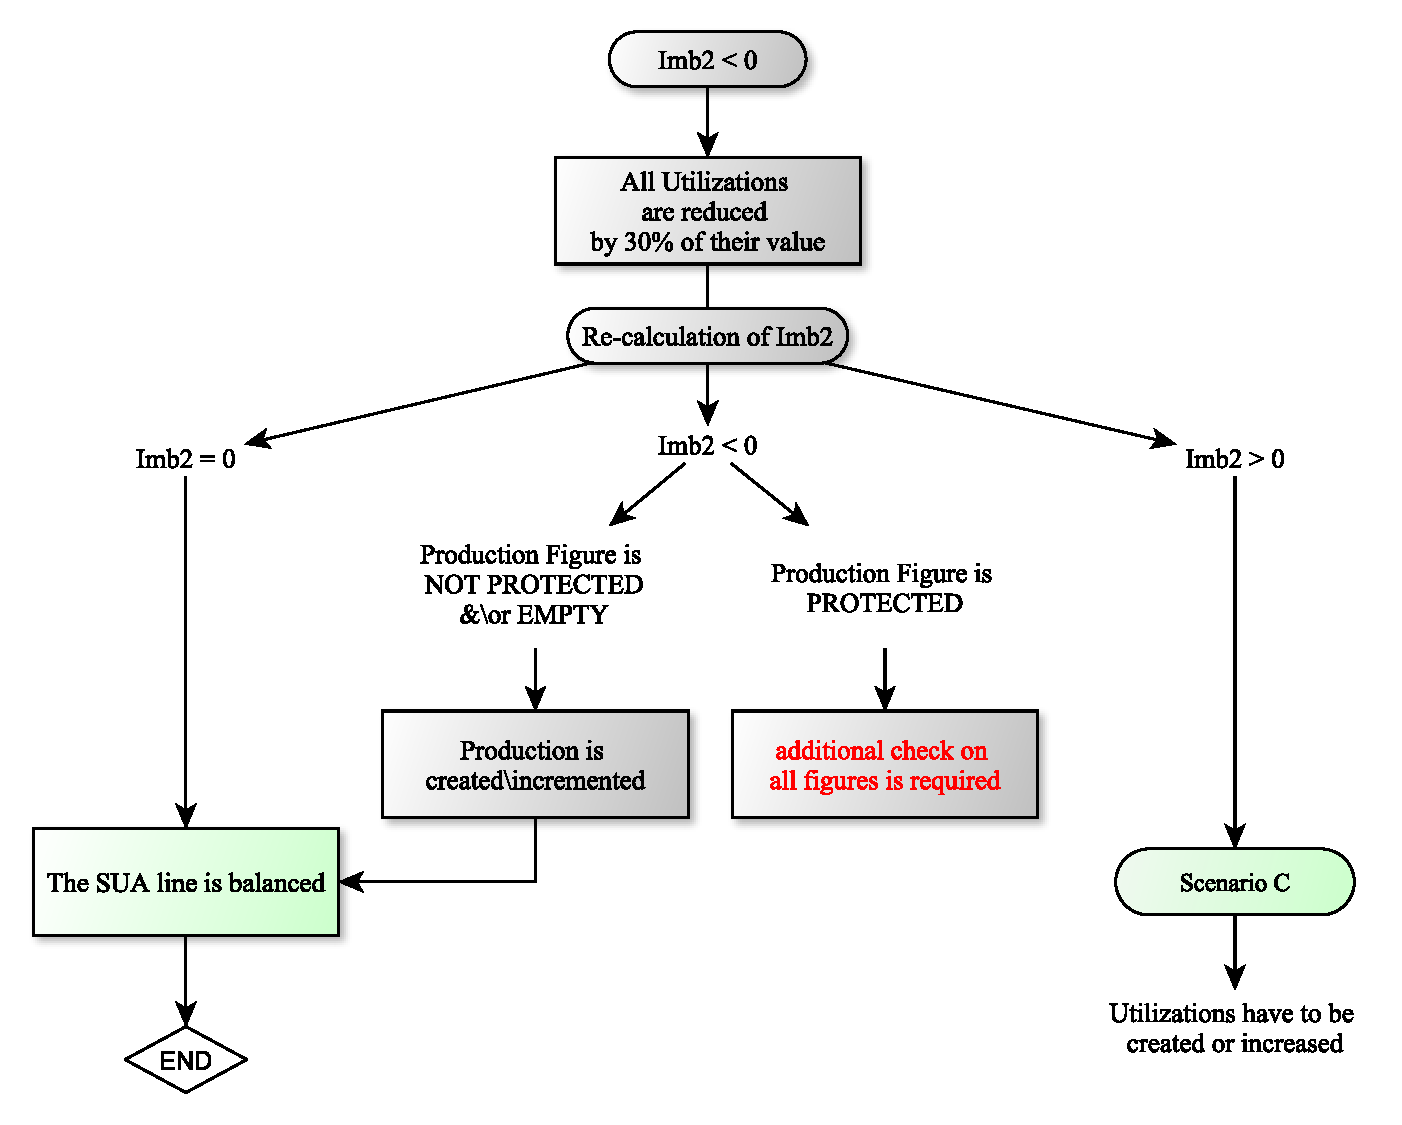
\includegraphics{images/06_NegativeImbalance} 

}

\caption{\label{fig:f5}Workflow of Sua Filling when there is a negative imbalance}\label{fig:f6}
\end{figure}

\begin{landscape}\begin{table}

\caption{\label{tab:t7}Sua table with utilizations filled (Example China Mainland, Wheat 2014)}
\centering
\resizebox{\linewidth}{!}{\fontsize{18}{20}\selectfont
\begin{tabular}[t]{>{\raggedleft\arraybackslash}p{10em}|l|>{\raggedright\arraybackslash\leavevmode\color{black}}p{6em}|>{\raggedright\arraybackslash\leavevmode\color{black}}p{6em}|>{\raggedright\arraybackslash\leavevmode\color{black}}p{6em}|>{\raggedright\arraybackslash\leavevmode\color{black}}p{6em}|>{\raggedright\arraybackslash\leavevmode\color{black}}p{6em}|>{\raggedright\arraybackslash\leavevmode\color{black}}p{6em}|>{\raggedright\arraybackslash\leavevmode\color{black}}p{6em}|>{\raggedright\arraybackslash\leavevmode\color{black}}p{6em}|>{\raggedright\arraybackslash\leavevmode\color{black}}p{6em}|>{\raggedright\arraybackslash\leavevmode\color{black}}p{6em}|>{\raggedright\arraybackslash\leavevmode\color{black}}p{6em}|>{\bfseries\em\leavevmode\color{red}}l}
\hline
\multicolumn{1}{r}{\textbf{itemName}} & \multicolumn{1}{c}{\textbf{P}} & \multicolumn{1}{c}{\textbf{I}} & \multicolumn{1}{c}{\textbf{X}} & \multicolumn{1}{c}{\textbf{DSt}} & \multicolumn{1}{c}{\textbf{Fo}} & \multicolumn{1}{c}{\textbf{FP}} & \multicolumn{1}{c}{\textbf{Fe}} & \multicolumn{1}{c}{\textbf{Se}} & \multicolumn{1}{c}{\textbf{T}} & \multicolumn{1}{c}{\textbf{IU}} & \multicolumn{1}{c}{\textbf{L}} & \multicolumn{1}{c}{\textbf{ROU}} & \multicolumn{1}{c}{\textbf{Imb2}}\\
\hline
Wheat & 126,208,400 & 2,971,249 & 957 & 1,120,565 &  & 90,384,615 & 29,181,617 & 4,277,567 &  & 2,985,279 & 2,713,000 & - & -1,483,951\\
\hline
Wheat and meslin flo & 70,500,000 & 33,055 & 188,674 &  & **68,372,646** & 1,958,146 &  &  & **-17,621** &  &  & - & 0\\
\hline
Mixes and doughs for &  & 6,497 & 38,072 &  & 0 &  & 0 &  & 0 &  &  & - & -31,575\\
\hline
Other Fructose and S & 158,665 & 3,659 & 162,324 &  & 0 &  &  &  & 0 &  &  & - & 0\\
\hline
Starch of Wheat & **314,020** & 11,035 & 40,311 &  &  & 158,664 & **120,537** &  &  & **5,543** &  & - & 0\\
\hline
Wheat Gluten & 116,496 & 877 & 117,373 &  &  & 0 & 0 &  &  &  &  & - & 0\\
\hline
Communion wafers & 13,263 & 8,796 & 5,822 &  & 16,241 &  &  &  & -4 &  &  & - & 0\\
\hline
Uncooked pasta & 1,415,692 & 12,520 & 22,550 &  & **1,406,024** &  &  &  & **-363** &  &  & - & 0\\
\hline
Food Preparations of &  & 69,686 & 21,977 &  & 47,709 &  &  &  & -12 &  &  & - & 12\\
\hline
Bran of Wheat & 21,414,279 & 156,359 & 2,200 &  & **16,689,929** &  & **4,882,810** &  & **-4,301** &  &  & - & 0\\
\hline
Gluten Feed and Meal & 793,740 & 160,230 & 529,333 &  &  &  & **424,637** &  &  &  &  & - & 0\\
\hline
bread & 15,485 & 2,897 & 4,210 &  & 14,175 &  &  &  & -3 &  &  & - & 0\\
\hline
pastry & 193,950 & 89,593 & 117,630 &  & **165,957** &  &  &  & **-42.75** &  &  & - & 0\\
\hline
\multicolumn{14}{l}{\textsuperscript{*} P=Production, I=Import, X=Export, DSt=Delta Stock, Fo=Food Availability, FP=FoodProcessing, Fe=Feed, Se=Seed, T=Tourism Consumption, IU=IndustrialUse, L=Loss,}\\
\multicolumn{14}{l}{ROU=Residual and other uses}\\
\end{tabular}}
\end{table}
\end{landscape}

\subsubsection*{\texorpdfstring{\emph{Imbalance \textgreater{} 0
(Scenario
C)}}{Imbalance \textgreater{} 0 (Scenario C)}}\label{imbalance-0-scenario-c}
\addcontentsline{toc}{subsubsection}{\emph{Imbalance \textgreater{} 0
(Scenario C)}}

When \(Imb2 >0\) there is an excess of supply that has to be distributed
trought utilizations. Here:

\begin{itemize}
\tightlist
\item
  A \emph{Utilization Table} tells which figures are supposed to be
  filled.
\item
  The Imbalance is distributed among variables according to a, so
  called, \emph{Multiple Filler approach} which make use of the
  \emph{Inverse Ranking Rule}.
\end{itemize}

\subsubsection*{\texorpdfstring{--\textgreater{} The \emph{Utilization
table}}{--\textgreater{} The Utilization table}}\label{the-utilization-table}
\addcontentsline{toc}{subsubsection}{--\textgreater{} The
\emph{Utilization table}}

Utilization table is a Country/commodity table telling which
Utilizations historically have been active for each commodity and
assigning a Rank and an inverse rank to each utilization based on its
mean value over the period 2000-2013. Table 9 shows the Utilization
table for \emph{Wheat and meslin flour} in China Mainland.

\begin{longtable}[]{@{}ccccc@{}}
\caption{Utilization Table Wheat and meslin Flour China Mainland
2014}\tabularnewline
\toprule
AreaM49 & Element & ItemCpc & rank & rankInv\tabularnewline
\midrule
\endfirsthead
\toprule
AreaM49 & Element & ItemCpc & rank & rankInv\tabularnewline
\midrule
\endhead
1248 & FP & 23110 & 2 & 3\tabularnewline
1248 & Fo & 23110 & 1 & 4\tabularnewline
1248 & DSt & 23110 & 4 & 1\tabularnewline
1248 & X & 23110 & 3 & 2\tabularnewline
\bottomrule
\end{longtable}

Where \(1248\) is the m49 code for China Mainland and \(23110\) is the
cpc code of Wheat and Meslin Flour. The table tells the following
information:

\begin{enumerate}
\def\labelenumi{\arabic{enumi}.}
\tightlist
\item
  The reported commodity in China, as been historically used:

  \begin{itemize}
  \tightlist
  \item
    for producing other commodities (\emph{Food Processing}),
  \item
    for human consumption (\emph{Food}),
  \item
    for increasing stocks (\emph{Stock Variation}),
  \item
    for exports (\emph{exports}).
  \end{itemize}
\item
  The biggest amount of availability of the reported commodity was used
  for Human consumption, the second big for processing other commodity,
  then for exports and, in the end, for increasing stocks.
\end{enumerate}

These informations are combined with the amount of \emph{Imb2} for
filling the SUAs of each derived commodity according to a set of rules
all falling into the, so called, \emph{Multiple Filler approach}.

\subsubsection*{\texorpdfstring{--\textgreater{} The \emph{Multiple
Filler Approach} and the \emph{Inverse Ranking
Rule}}{--\textgreater{} The Multiple Filler Approach and the Inverse Ranking Rule}}\label{the-multiple-filler-approach-and-the-inverse-ranking-rule}
\addcontentsline{toc}{subsubsection}{--\textgreater{} The \emph{Multiple
Filler Approach} and the \emph{Inverse Ranking Rule}}

This approach distribute the \(Imb2\) across utilizations, by the ules
reported in Figure \ref{fig:f7}.

\begin{figure}

{\centering 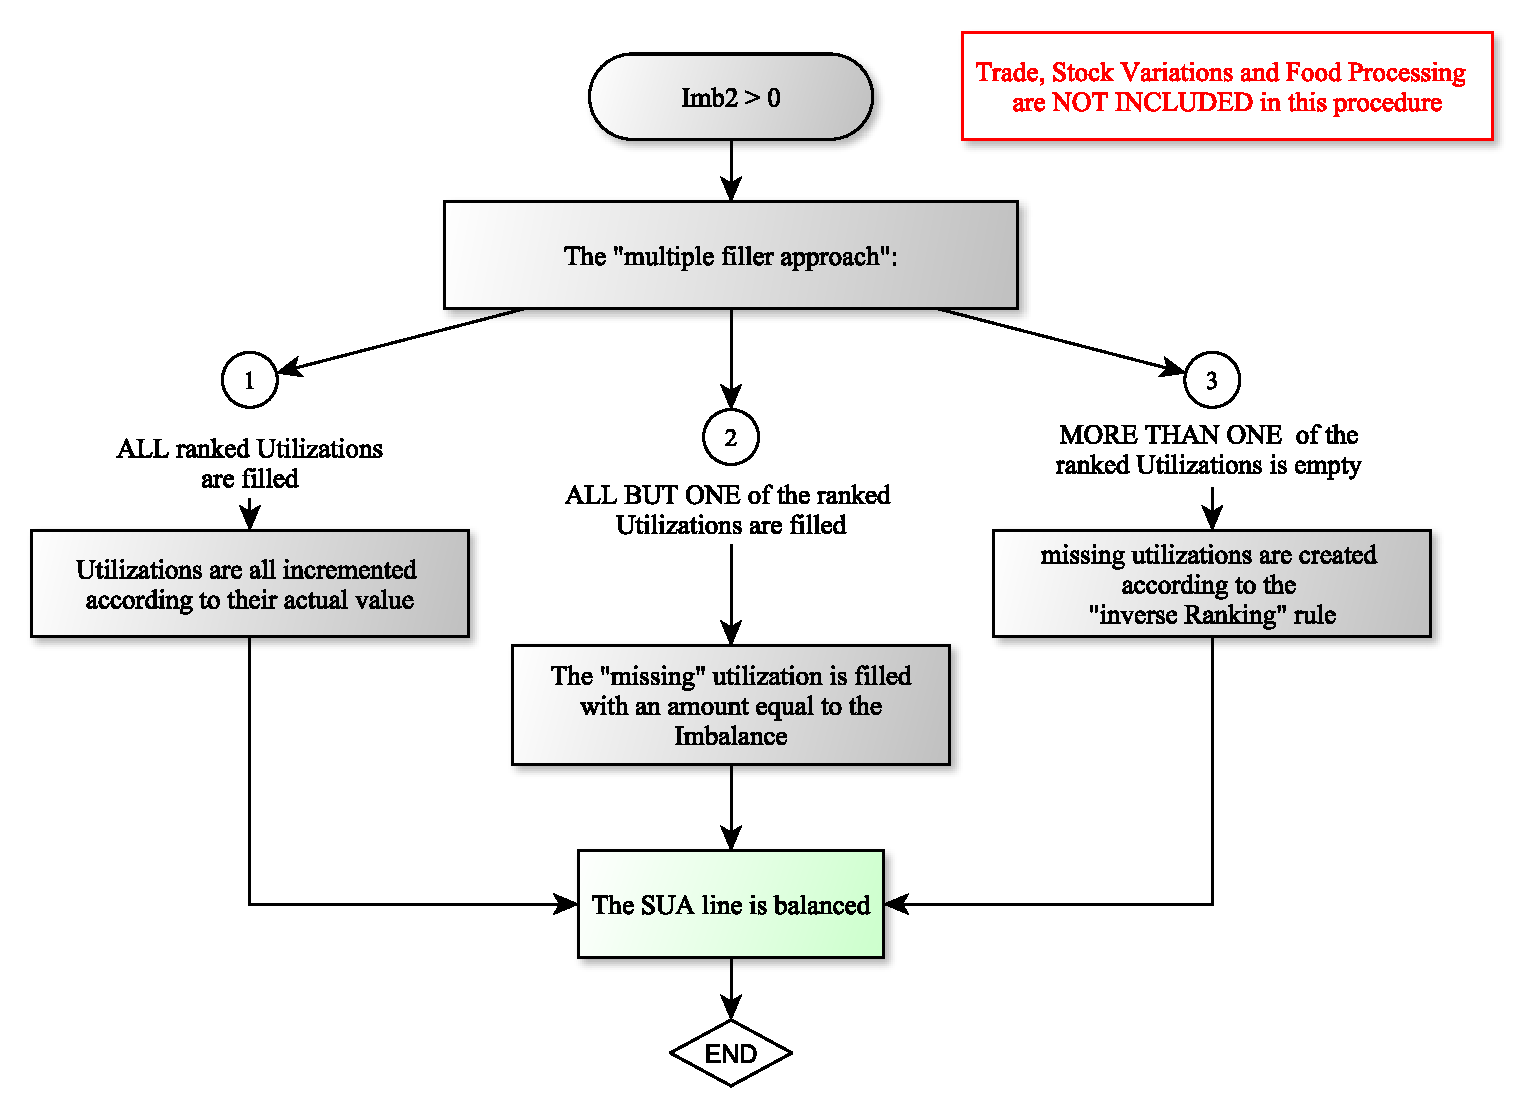
\includegraphics{images/07_PositiveImbalance} 

}

\caption{\label{fig:f5}Workflow of Sua Filling when there is a positive imbalance}\label{fig:f7}
\end{figure}

As reported in the Figure, Three cases may happen:

\begin{enumerate}
\def\labelenumi{\arabic{enumi}.}
\tightlist
\item
  If all the ranked utilizations are already filled, all of them are
  increased proportionally to their values. \emph{Bran of Wheat} in our
  example, belongs to this case. Utilization table for Bran of Wheat is
  reported in Table 10
\end{enumerate}

\begin{longtable}[]{@{}ccccc@{}}
\caption{Utilization Table Bran ofWheat China Mainland
2014}\tabularnewline
\toprule
AreaM49 & Element & ItemCpc & rank & rankInv\tabularnewline
\midrule
\endfirsthead
\toprule
AreaM49 & Element & ItemCpc & rank & rankInv\tabularnewline
\midrule
\endhead
1248 & Fe & 39120.01 & 2 & 2\tabularnewline
1248 & Fo & 39120.01 & 1 & 3\tabularnewline
1248 & X & 39120.01 & 3 & 1\tabularnewline
\bottomrule
\end{longtable}

\begin{quote}
According to this table, there are 3 Utilizations that are suppose to be
active for this commodity: \emph{feed}, \emph{food} and \emph{exports}.
\emph{Exports} is excluded from this step, therefore, food and feed
reamain. Both Variables are filled in the SUA line of This Commodity,
therefore, all of them are increased proportionally to their values.
\end{quote}

\begin{enumerate}
\def\labelenumi{\arabic{enumi}.}
\setcounter{enumi}{1}
\item
  If all the ranked utilizations are already filled but one, the all
  imbalance goes to that commodity. In our Example, this is the case of
  \emph{Gluten Feed and meals} (Table 10).
\item
  Finally, if more that one utilization is empty, the so called
  \textbf{\emph{Inverse Ranking rule}} is activated. This rule assigns
  part of the imbalance to the ranked utilizations proportionally to the
  ranks. This happens by making use of the inverse rank of all the
  utilizations that are ``activable'' and not excluded from the
  procedure. The rule works for any number of ranks and independently
  from the number of utilizations that have to be excluded.
\end{enumerate}

\begin{quote}
The \emph{Inverse ranking rule} starts from the Utilization table with
the addition of a column containing the \emph{rank weigth \(Wr\)}, as
reported in the following table:
\end{quote}

\begin{quote}
\begin{center}
\begin{tabular}{ c|c|c|c } 
\hline
element ($Ut_{i}$) & rank ($r_{i}$) & Inverse rank ($Ir_{i}$) & weight Rank ($Wr_{i}$)\\
\hline
$Ut_{1}$ & $r_{1}$ & $Ir_{1}$  & $Wr_{1}$\\ 
... & ... & ... & ...\\ 
$Ut_{i}$ & $r_{i}$ & $Ir_{i}$  & $Wr_{i}$\\ 
... & ... & ... & ...\\ 
$Ut_{n}$ & $r_{n}$ & $Ir_{n}$  & $Wr_{n}$\\ 
\hline
\end{tabular}
\end{center}
\end{quote}

\begin{quote}
where:
\end{quote}

\begin{quote}
\begin{itemize}
\tightlist
\item
  \(Ut_{i}\) is the generic utilization, with \(i=1,2,...n\)
\item
  \(r_{i}\) is the rank of utilization \(Ut_{i}\), with \(i=1,2,...n\)
\item
  \(Ir_{i}\) is the Inverse rank of utilization \(Ut_{i}\), with
  \(i=1,2,...n\) and is equal to:
\end{itemize}
\end{quote}

\begin{quote}
\begin{quote}
\begin{equation}
\label{eq:inverseRankequation}
Ir_{i} = max(r)-r_{i}+1
\end{equation}
\end{quote}
\end{quote}

\begin{quote}
\begin{itemize}
\tightlist
\item
  \(Wr_{i}\) is the rank weight of utilization \(Ut_{i}\) and is equal
  to 0 or 1 depending on the element being, respectively, exluded or not
  from the sua filling (Table 11).
\end{itemize}
\end{quote}

\begin{longtable}[]{@{}cc@{}}
\caption{Rank Weight of the elements of FBS}\tabularnewline
\toprule
Utilizations & Wr\tabularnewline
\midrule
\endfirsthead
\toprule
Utilizations & Wr\tabularnewline
\midrule
\endhead
\(X\) & \(0\)\tabularnewline
\(DSt\) & \(0\)\tabularnewline
\(Fo\) & \(1\)\tabularnewline
\(FP\) & \(0\)\tabularnewline
\(Fe\) & \(1\)\tabularnewline
\(Se\) & \(1\)\tabularnewline
\(T\) & \(1\)\tabularnewline
\(IU\) & \(1\)\tabularnewline
\(L\) & \(1\)\tabularnewline
\(ROU\) & \(0\)\tabularnewline
\bottomrule
\end{longtable}

\begin{quote}
The value \(Value_{i}\) assigned to the utilization of each commodity is
calculated as a rank based proportion \(pR_{i}\) of the total \(Imb2\)
according to the following equation:
\end{quote}

\begin{quote}
\begin{equation}
\label{eq:inverseRank}
Value_{i} = Imb2 \times pR_{i}
\end{equation}
\end{quote}

\begin{quote}
with \(pR_{i}\) depending on \(\sum \limits_{i=1}^n Wr_{i}\):
\end{quote}

\begin{quote}
\begin{equation}
\label{eq:weightRank}
\begin{cases}
pR_{i} = 0     & \quad \text{when} \quad \sum \limits_{i=1}^n Wr_{i} = 0\\
pR_{i} = \frac{Ir_{i}\times we_{i}}{\sum \limits_{i=1}^n\left(Ir_{i}\times Wr_{i}\right)}     & \quad \text{when} \quad \sum \limits_{i=1}^n Wr_{i} > 0 
\end{cases}
\end{equation}
\end{quote}

\begin{quote}
\end{quote}

\begin{quote}
As an example consider the SUA line of \emph{Cocoa Beans} in Madagascar
in 2014 (Table 12) and the Utilization table of the same
country/commodity combination (Table 13)
\end{quote}

\begin{longtable}[]{@{}cccccccccccccc@{}}
\caption{Sua line of Cocoa Beans Madagascar 2014 - before Sua
Filling}\tabularnewline
\toprule
itemName & P & I & X & DSt & Fo & FP & Fe & Se & T & IU & L & ROU &
Imb2\tabularnewline
\midrule
\endfirsthead
\toprule
itemName & P & I & X & DSt & Fo & FP & Fe & Se & T & IU & L & ROU &
Imb2\tabularnewline
\midrule
\endhead
\emph{Cocoa beans} & 10,865 & 36 & 8,326 & - & - & - & - & - & - & - &
743 & - & \textbf{\emph{1,832}}\tabularnewline
\bottomrule
\end{longtable}

\begin{longtable}[]{@{}cccc@{}}
\caption{Utilization table for Cocoa Beans Madagascar}\tabularnewline
\toprule
Ut & r & Ir & Wr\tabularnewline
\midrule
\endfirsthead
\toprule
Ut & r & Ir & Wr\tabularnewline
\midrule
\endhead
FP & 4 & 2 & 0\tabularnewline
Fo & 2 & 4 & 1\tabularnewline
IU & 3 & 3 & 1\tabularnewline
DSt & 5 & 1 & 0\tabularnewline
X & 1 & 5 & 0\tabularnewline
\bottomrule
\end{longtable}

\begin{quote}
Besides the excluded elements, there are 2 utilizations empty:
\emph{food} and \emph{Industrial Use}. The Values of these two elements
is calculated as folows and the result shown in Table 14:
\end{quote}

\begin{quote}
\begin{equation}
\begin{aligned}
pR_{Fo} &= \frac{4\times 1}{0 + 0 + 4 + 3 + 0 + 0} = 4/7 = 0.57143 \\
Value_{Fo} &= 1,832 \times 0.57143 = 1,047 
\end{aligned}
\end{equation}
\end{quote}

\begin{quote}
\end{quote}

\begin{quote}
\begin{equation}
\begin{aligned}
\label{eq:VIUC}
pR_{IU} &= \frac{3\times 1}{0 + 0 + 4 + 3 + 0 + 0} = 3/7 = 0.42857\\
Value_{IU} &= 1,832 \times 0.42857 = 785
\end{aligned}
\end{equation}
\end{quote}

\begin{longtable}[]{@{}cccccccccccccc@{}}
\caption{Sua line of Cocoa Beans Madagascar 2014 - after Sua
Filling}\tabularnewline
\toprule
itemName & P & I & X & DSt & Fo & FP & Fe & Se & T & IU & L & ROU &
Imb2\tabularnewline
\midrule
\endfirsthead
\toprule
itemName & P & I & X & DSt & Fo & FP & Fe & Se & T & IU & L & ROU &
Imb2\tabularnewline
\midrule
\endhead
\emph{Cocoa beans} & 10,865 & 36 & 8326 & - & \textbf{\emph{1,047}} & -
& - & - & - & \textbf{\emph{785}} & 743 & - &
\textbf{\emph{0}}\tabularnewline
\bottomrule
\end{longtable}

\subsection{The Sua Balanced}\label{the-sua-balanced}

The table resulting after the Sua Filling is called \emph{Sua Balanced}.
For the Example of China Mainland, wheat 2014 the \emph{Sua Balanced} is
reported in Table 15

\begin{landscape}\begin{table}

\caption{\label{tab:t14}Sua Balanced (Example China Mainland, Wheat 2014)}
\centering
\resizebox{\linewidth}{!}{\fontsize{18}{20}\selectfont
\begin{tabular}[t]{r|l|l|l|l|l|l|l|l|l|l|l|l|l}
\hline
\multicolumn{1}{r}{\textbf{itemName}} & \multicolumn{1}{c}{\textbf{P}} & \multicolumn{1}{c}{\textbf{I}} & \multicolumn{1}{c}{\textbf{X}} & \multicolumn{1}{c}{\textbf{DSt}} & \multicolumn{1}{c}{\textbf{Fo}} & \multicolumn{1}{c}{\textbf{FP}} & \multicolumn{1}{c}{\textbf{Fe}} & \multicolumn{1}{c}{\textbf{Se}} & \multicolumn{1}{c}{\textbf{T}} & \multicolumn{1}{c}{\textbf{IU}} & \multicolumn{1}{c}{\textbf{L}} & \multicolumn{1}{c}{\textbf{ROU}} & \multicolumn{1}{c}{\textbf{Imb2}}\\
\hline
\textcolor{red}{\em{\textbf{Wheat}}} & \textcolor{red}{\em{\textbf{126,208,400}}} & \textcolor{red}{\em{\textbf{2,971,249}}} & \textcolor{red}{\em{\textbf{957}}} & \textcolor{red}{\em{\textbf{1,120,565}}} & \textcolor{red}{\em{\textbf{}}} & \textcolor{red}{\em{\textbf{90,384,615}}} & \textcolor{red}{\em{\textbf{29,181,617}}} & \textcolor{red}{\em{\textbf{4,277,567}}} & \textcolor{red}{\em{\textbf{}}} & \textcolor{red}{\em{\textbf{2,985,279}}} & \textcolor{red}{\em{\textbf{2,713,000}}} & \textcolor{red}{\em{\textbf{-}}} & \textcolor{red}{\em{\textbf{-1,483,951}}}\\
\hline
Wheat and meslin flo & 70,500,000 & 33,055 & 188,674 &  & 68,372,646 & 1,958,146 &  &  & -17,621 &  &  & - & 0\\
\hline
\textcolor{red}{\em{\textbf{Mixes and doughs for}}} & \textcolor{red}{\em{\textbf{}}} & \textcolor{red}{\em{\textbf{6,497}}} & \textcolor{red}{\em{\textbf{38,072}}} & \textcolor{red}{\em{\textbf{}}} & \textcolor{red}{\em{\textbf{0}}} & \textcolor{red}{\em{\textbf{}}} & \textcolor{red}{\em{\textbf{0}}} & \textcolor{red}{\em{\textbf{}}} & \textcolor{red}{\em{\textbf{0}}} & \textcolor{red}{\em{\textbf{}}} & \textcolor{red}{\em{\textbf{}}} & \textcolor{red}{\em{\textbf{-}}} & \textcolor{red}{\em{\textbf{-31,575}}}\\
\hline
Other Fructose and S & 158,665 & 3,659 & 162,324 &  & 0 &  &  &  & 0 &  &  & - & 0\\
\hline
Starch of Wheat & 314,020 & 11,035 & 40,311 &  &  & 158,664 & 120,537 &  &  & 5,543 &  & - & 0\\
\hline
Wheat Gluten & 116,496 & 877 & 117,373 &  &  & 0 & 0 &  &  &  &  & - & 0\\
\hline
Communion wafers & 13,263 & 8,796 & 5,822 &  & 16,241 &  &  &  & -4 &  &  & - & 0\\
\hline
Uncooked pasta & 1,415,692 & 12,520 & 22,550 &  & 1,406,024 &  &  &  & -363 &  &  & - & 0\\
\hline
\textcolor{red}{\em{\textbf{Food Preparations of}}} & \textcolor{red}{\em{\textbf{}}} & \textcolor{red}{\em{\textbf{69,686}}} & \textcolor{red}{\em{\textbf{21,977}}} & \textcolor{red}{\em{\textbf{}}} & \textcolor{red}{\em{\textbf{47,709}}} & \textcolor{red}{\em{\textbf{}}} & \textcolor{red}{\em{\textbf{}}} & \textcolor{red}{\em{\textbf{}}} & \textcolor{red}{\em{\textbf{-12}}} & \textcolor{red}{\em{\textbf{}}} & \textcolor{red}{\em{\textbf{}}} & \textcolor{red}{\em{\textbf{-}}} & \textcolor{red}{\em{\textbf{12}}}\\
\hline
Bran of Wheat & 21,414,279 & 156,359 & 2,200 &  & 16,689,929 &  & 4,882,810 &  & -4,301 &  &  & - & 0\\
\hline
Gluten Feed and Meal & 793,740 & 160,230 & 529,333 &  &  &  & 424,637 &  &  &  &  & - & 0\\
\hline
bread & 15,485 & 2,897 & 4,210 &  & 14,175 &  &  &  & -3 &  &  & - & 0\\
\hline
pastry & 193,950 & 89,593 & 117,630 &  & 165,957 &  &  &  & -42.75 &  &  & - & 0\\
\hline
\multicolumn{14}{l}{\textsuperscript{*} P=Production, I=Import, X=Export, DSt=Delta Stock, Fo=Food Availability, FP=FoodProcessing, Fe=Feed, Se=Seed, T=Tourism Consumption, IU=IndustrialUse, L=Loss,}\\
\multicolumn{14}{l}{ROU=Residual and other uses}\\
\end{tabular}}
\end{table}
\end{landscape}

The red lines are not balanced lines. Indeed, the \emph{Sua Filling}
procedure does not interveene on all the commodities. It leaves
unbalanced all the ``top level'' commodities falling in 2 main
categories:

\begin{enumerate}
\def\labelenumi{\arabic{enumi}.}
\tightlist
\item
  The \emph{Primary commodities}. These are all the crop commodities,
  like cereals, pulses, vegetables, fruits etc, that are often processed
  in other commodities, like the wheat in flour of wheat.
\item
  The \emph{no tree} commodities. These commodities are excluded from
  the list of commodities that are processed into something else, they
  are often mixes of some other crop or commodity and used for specific
  purposes, i.e. \emph{Mixes and dough for the preparation of baker's
  wares} and \emph{Food preparations of Flour, Meal or Malt Extract}
  from our example.
\end{enumerate}

Therefore 3 lines are not balanced in Table 15, belonging to these 2
categories of ``not balanced'' commodities.

The reason for the exclusion of the \emph{zero-level} commodities form
the filling stays in the circumstance for which the standardization will
affect the figures of the primary commodities, this opening the need for
a final \emph{balancing} procedure. In order not to intervene twice on
these commodities, it has been decide to keep as smaller as possible the
number correction, so to reduce error.

\section{The Standardization}\label{the-standardization}

The \emph{Standardization} is the process of transforming all the
processed commodities in terms of their primary commodities, so to have
all the existing food availability of a country, expressed in terms of
the main commodities. Aggregation of data from a detailed product
classification to a more comprehensive one is common practice for two
reasons. The first reason is to reduce the amount of data, and the
number of commodities involved, to a level and size more suited for
analytical purposes. The second reason is, that by cancelling out the
intermediate production of derived products against the input use of
primary products, a clearer view emerges of the domestic availability of
a product and its final uses.


\end{document}
